\documentclass{amsart}

\usepackage[T1]{fontenc}
\usepackage{amsmath, amsfonts, amssymb, amsthm, mathrsfs, wasysym, graphics, graphicx, xcolor, url, hyperref, hypcap, xargs, multicol, pdflscape, multirow, hvfloat, array, ae, aecompl, pifont, mathtools, a4wide, float, blkarray, overpic, nicefrac}
\usepackage[shortlabels, inline]{enumitem}%shortlabels to have same syntax as enumerate package, inline gives inline option with *
\usepackage{bbm}%allows for \mathbbm{1}
\usepackage[noabbrev,capitalise]{cleveref}
\usepackage[normalem]{ulem}
\usepackage{marginnote}
\hypersetup{colorlinks=true, citecolor=darkblue, linkcolor=darkblue}
\usepackage[all]{xy}
\usepackage{tikz}
\usepackage{tikz-cd}
%\usepackage{tkz-graph}
\usetikzlibrary{trees, decorations, decorations.pathmorphing, decorations.markings, decorations.shapes, shapes, arrows, matrix, calc, fit, intersections, patterns, angles}
\graphicspath{{figures/}{figures/diagonals/}{figures/walks/}{figures/tubes/}{figures/blocks/}}
\makeatletter\def\input@path{{figures/}}\makeatother
\usepackage{caption}
\captionsetup{width=\textwidth}
\usepackage[export]{adjustbox}

%%%%%%%%%%%%%%%%%%%%%%%%%%%%%%%%%%%%%%

% STANDARD

% theorems
\newtheorem{theorem}{Theorem}[section]
\newtheorem{corollary}[theorem]{Corollary}
\newtheorem{proposition}[theorem]{Proposition}
\newtheorem{lemma}[theorem]{Lemma}
\newtheorem{conjecture}[theorem]{Conjecture}
\newtheorem*{theorem*}{Theorem}%[section]

\theoremstyle{definition}
\newtheorem{definition}[theorem]{Definition}
\newtheorem{example}[theorem]{Example}
\newtheorem{remark}[theorem]{Remark}
\newtheorem{question}[theorem]{Question}
\newtheorem{notation}[theorem]{Notation}
\newtheorem{assumption}[theorem]{Assumption}
\newtheorem{convention}[theorem]{Convention}

\crefname{equation}{Equation}{Equations}

% math special letters
\newcommand{\R}{\mathbb{R}} % reals
\newcommand{\Q}{\mathbb{Q}} % rationals
\newcommand{\N}{\mathbb{N}} % naturals
\newcommand{\Z}{\mathbb{Z}} % integers
\newcommand{\C}{\mathbb{C}} % complex
\newcommand{\I}{\mathbb{I}} % set of integers
\newcommand{\K}{k} % field
\newcommand{\bb}[1]{{\mathbb{#1}}} % mathbb letters
\newcommand{\f}[1]{{\mathfrak{#1}}} % mathfrak letters
\renewcommand{\c}[1]{{\mathcal{#1}}} % call letters
\renewcommand{\b}[1]{{\boldsymbol{#1}}} % bold letters
\newcommand{\h}{\widehat} % hat letters

% math commands
\newcommand{\set}[2]{\left\{ #1 \;\middle|\; #2 \right\}} % set notation
\newcommand{\bigset}[2]{\big\{ #1 \;\big|\; #2 \big\}} % big set notation
\newcommand{\Bigset}[2]{\Big\{ #1 \;\Big|\; #2 \Big\}} % Big set notation
\newcommand{\setangle}[2]{\left\langle #1 \;\middle|\; #2 \right\rangle} % set notation
\newcommand{\ssm}{\smallsetminus} % small set minus
\newcommand{\dotprod}[2]{\langle \, #1 \; | \; #2 \, \rangle} % dot product
\newcommand{\bigdotprod}[2]{\big\langle \, #1 \; \big| \; #2 \, \big\rangle} % dot product
\newcommand{\symdif}{\,\triangle\,} % symmetric difference
\newcommand{\one}{\mathbbm{1}} % the all one vector
\newcommandx{\ones}[1][1=n]{\one_{#1}} % the all one vector of length n
\newcommand{\eqdef}{\mbox{\,\raisebox{0.2ex}{\scriptsize\ensuremath{\mathrm:}}\ensuremath{=}\,}} % :=
\newcommand{\defeq}{\mbox{~\ensuremath{=}\raisebox{0.2ex}{\scriptsize\ensuremath{\mathrm:}} }} % =:
\newcommand{\simplex}{\triangle} % simplex
\renewcommand{\implies}{\Rightarrow} % imply sign
\newcommand{\transpose}[1]{{#1}^T} % transpose matrix
\newcommand{\truth}[1]{\left[ #1 \right]} % truth (kronecker delta)

% operators
\DeclareMathOperator{\conv}{conv} % convex hull
\DeclareMathOperator{\vect}{vect} % linear span
\DeclareMathOperator{\cone}{cone} % cone hull

% others
\newcommand{\ie}{\textit{i.e.}~} % id est
\newcommand{\eg}{\textit{e.g.}~} % exempli gratia
\newcommand{\Eg}{\textit{E.g.}~} % exempli gratia
\newcommand{\apriori}{\textit{a priori}} % a priori
\newcommand{\viceversa}{\textit{vice versa}} % vice versa
\newcommand{\versus}{\textit{vs.}~} % versus
\newcommand{\aka}{\textit{a.k.a.}~} % also known as
\newcommand{\perse}{\textit{per se}} % per se
\newcommand{\ordinal}{\textsuperscript{th}} % th for ordinals
\newcommand{\ordinalst}{\textsuperscript{st}} % st for ordinals
\definecolor{darkblue}{rgb}{0,0,0.7} % darkblue color
\definecolor{green}{RGB}{57,181,74} % green color
\definecolor{violet}{RGB}{147,39,143} % violet color
\newcommand{\red}{\color{red}} % red command
\newcommand{\blue}{\color{blue}} % blue command
\newcommand{\orange}{\color{orange}} % orange command
\newcommand{\green}{\color{green}} % green command
\newcommand{\darkblue}{\color{darkblue}} % darkblue command
\newcommand{\defn}[1]{\textsl{\darkblue #1}} % emphasis of a definition
\newcommand{\para}[1]{\medskip\noindent\uline{\textit{#1.}}} % paragraph
\renewcommand{\topfraction}{1} % possibility to have one page of pictures
\renewcommand{\bottomfraction}{1} % possibility to have one page of pictures
\newcommand{\shade}[1]{{\color{cyan} #1}}

% marginal comments
\usepackage{todonotes}
\newcommand{\guillaume}[1]{\todo[color=orange!30]{#1 --- G.}}
\newcommand{\vincent}[1]{\todo[color=blue!30]{#1 \\ \hfill --- V.}}

% formating the part command
\makeatletter
\def\part{\@startsection{part}{1}%
\z@{.7\linespacing\@plus\linespacing}{.8\linespacing}%
{\LARGE\sffamily\centering}}
%\@addtoreset{section}{part}
\makeatother
\renewcommand{\thepart}{\Roman{part}}
%\renewcommand{\thesection}{\arabic{part}.\arabic{section}}

% formating the table of contents
\setcounter{tocdepth}{4}
\makeatletter
\def\l@section{\@tocline{1}{5pt}{0pc}{}{}}
\makeatother
\let\oldtocpart=\tocpart
\renewcommand{\tocpart}[2]{\sc\large\oldtocpart{#1}{#2}}
\let\oldtocsection=\tocsection
\renewcommand{\tocsection}[2]{\bf\oldtocsection{#1}{#2}}
\let\oldtocsubsubsection=\tocsubsubsection
\renewcommand{\tocsubsubsection}[2]{\quad\oldtocsubsubsection{#1}{#2}}

% drapeau européen
\usepackage{graphicx,calc}
\newlength\myheight
\newlength\mydepth
\settototalheight\myheight{Xygp}
\settodepth\mydepth{Xygp}
\setlength\fboxsep{0pt}
\newcommand*\inlinegraphics[1]{%
  \settototalheight\myheight{Xygp}%
  \settodepth\mydepth{Xygp}%
  \raisebox{-\mydepth}{\includegraphics[height=\myheight]{#1}}%
}

% SPECIFIC BLOCK GRAPH PERMUTREES

% COMBINATORICS

% decorations
\newcommand{\vertexSet}{V}
\newcommand{\decoration}{\delta}
\newcommandx{\Up}[2][1=v, 2=\decoration]{\smash{\overline #2}(#1)} 
\newcommandx{\Down}[2][1=v, 2=\decoration]{\smash{\underline #2}(#1)} 
\newcommandx{\up}[1][1=v]{\overline{#1}} 
\newcommandx{\down}[1][1=v]{\underline{#1}} 
\newcommandx{\updown}[1][1=v]{\overline{\underline{#1}}} 
% source and target
\newcommandx{\so}[1][1=i]{\textsc{s}_{#1}} % source set
\newcommandx{\ta}[1][1=o]{\textsc{t}_{#1}} % target set
% spines
\newcommandx{\spine}[1][1=S]{#1} % spine
\newcommandx{\almostSpine}[1][1=S]{\smash{\widetilde{#1}}} % spine
\newcommandx{\spines}[1][1=\b{G}]{\mathcal{S}(#1)} % set of spines
\newcommandx{\spinePoset}[1][1=\b{G}]{\mathcal{P}_{#1}} % spine poset
\newcommand{\blossom}{^\text{\ding{96}}} % blossom
\newcommand{\labeling}{\lambda} % labels in blossoming trees
\newcommandx{\equivalenceSpines}[2][1=\b{G}, 2=\b{G}']{\equiv_{#1 \to #2}} % equivalence relation on spines
% nested complex
\newcommandx{\nested}[1][1=N]{#1} % nested set
\newcommand{\negNested}{\preceq} % negative nested
\newcommand{\posNested}{\succeq} % positive nested
\newcommand{\negDisjoint}{\perp} % negative disjoint
\newcommand{\posDisjoint}{\;\top\;} % positive disjoint
\newcommandx{\nestedComplex}[1][1=\b{G}]{\mathcal{N}_{#1}} % nested complex
% maps
\newcommand{\spineToNested}{\mathsf{N}} % spine to nested set
\newcommand{\nestedToSpine}{\mathsf{S}} % nested set to spine
\newcommand{\partitionToSpine}{\mathsf{S}} % partition to spine
\newcommandx{\surjectionSpines}[2][1=\b{G}, 2=\b{G}']{\Phi_{#1 \to #2}} % spine to spine
\newcommand{\nodeSurj}[2]{\smash{n_{#1}^{#2}}} % node surjection
\newcommand{\arcSurj}[2]{\smash{\varepsilon_{#1}^{#2}}} % arc surjection
% insertion
\newcommand{\insertion}[2]{#1 \ll #2} % insertion

% GEOMETRY

% fans
\newcommand{\primalCone}{\mathsf{C}^\star} % primal cone
\newcommand{\normalCone}{\mathsf{C}} % normal cone
\newcommandx{\braidFan}[1][1=G]{\mathcal{F}_{#1}} % braid fan
\newcommandx{\sylvesterFan}[1][1=G]{\mathcal{T}_{#1}} % sylvester fan
\newcommandx{\graphicalFan}[1][1=G]{\mathcal{G}_{#1}} % graphical fan
\newcommandx{\spineFan}[1][1=\b{G}]{\mathcal{S}_{#1}} % spine fan
% polytopes
\newcommand{\polytope}[1]{\mathsf{#1}} % font polytopes
\newcommandx{\Perm}[2][1=G,2=\weight]{\polytope{Perm}^{#2}_{#1}} % permutahedron
\newcommandx{\Asso}[2][1=G,2=\weight]{\polytope{Asso}^{#2}_{#1}} % associahedron
\newcommandx{\Spin}[2][1=\b{G},2=\weight]{\polytope{Spin}^{#2}_{#1}} % spine polytope
\newcommandx{\Zono}[2][1=G,2=\weight]{\mathsf{Zono}^{#2}_{#1}} % zonotope
\newcommandx{\point}[2][1=\spine,2=\weight]{\b{a}^{#2}_{#1}} % point
\newcommand{\weight}{\omega} % weight
\newcommandx{\boundary}[1][1=\pi]{\partial#1} % endpoints of a path
\newcommandx{\peaks}[1][1=\pi]{\wedge#1} % top of a path
\newcommandx{\valleys}[1][1=\pi]{\vee#1} % bottom of a path
\newcommandx{\Hyp}[1][1=\weight]{\mathbf{H}^{= #1}} % hyperplane
\newcommandx{\HS}[1][1=\weight]{\mathbf{H}^{\ge #1}} % halfspace
\newcommand{\monombinom}[1]{\big\{\!\begin{smallmatrix} #1 \\ 2 \end{smallmatrix}\!\big\}}

%%%%%%%%%%%%%%%%%%%%%%%%%%%%%%%%%%%%%%

\title{Spine polytopes}

\author{Guillaume Laplante-Anfossi}
\address[Guillaume Laplante-Anfossi]{Universit\'e Sorbonne Paris Nord, Laboratoire Analyse, G\'eom\'etrie et Applications, CNRS, UMR 7539, F-93430 Villetaneuse, France}
\email{laplante-anfossi@math.univ-paris13.fr}
\urladdr{\url{https://www.math.univ-paris13.fr/~laplante-anfossi/}}

\author{Vincent Pilaud}
\address[Vincent Pilaud]{CNRS \& LIX, \'Ecole Polytechnique, Palaiseau}
\email{vincent.pilaud@lix.polytechnique.fr}
\urladdr{\url{http://www.lix.polytechnique.fr/~pilaud/}}

%\date{\today}

\subjclass[2010]{Primary 52B11; Secondary 18M70} 

%\keywords{Polytopes...}

\thanks{The first author was supported by the European Union's Horizon 2020 research and innovation program under the Marie Sklodowska-Curie grant agreement No 754362 \inlinegraphics{EU.png}, by the Natural Sciences and Engineering Research Council of Canada (NSERC) and by the ANR-20-CE40-0016 Higher Algebra, Geometry and Topology. The second author is supported by the French ANR grants CAPPS~17\,CE40\,0018, and CHARMS~19\,CE40\,0017.}

%%%%%%%%%%%%%%%%%%%%%%%%%%%%%%%%%%%%%%
%%%%%%%%%%%%%%%%%%%%%%%%%%%%%%%%%%%%%%%

\begin{document}

\begin{abstract}
TBC
\end{abstract}

\maketitle

\tableofcontents

%%%%%%%%%%%%%%%%%%%%%%%%%%%%%%%%%%%%%%%
%%%%%%%%%%%%%%%%%%%%%%%%%%%%%%%%%%%%%%%

\newpage
\section*{Introduction}

Common generalization of \cite{Pilaud-signedTreeAssociahedraFPSAC, LangePilaud, PilaudPons-permutrees, Laplante-diagonalOperahedra}.
It is the maximal generalization, according to \cite{Pilaud-removahedra}.

\guillaume{dioperads and string topology}
\guillaume{our dioperad might be initial in some operadic / Feynman / moment category}

%%%%%%%%%%%%%%%%%%%%%%%%%%%%%%%%%%%%%%%
%%%%%%%%%%%%%%%%%%%%%%%%%%%%%%%%%%%%%%%

\newpage
\section{Combinatorics: Spine Poset and Nested Complex}
\label{sec:combinatorics}

This section is dedicated to the combinatorics of spines on decorated block graphs.

%%%%%%%%%%%%%%%%%%%%%%%%%%%%%%%%%%%%%%%

\subsection{Maple trees and block graphs}
\label{subsec:MapleTreesBlockGraphs}

We start by defining the ground sets of our constructions.
We will use both maple trees and block graphs, which essentially encode the same information.

\begin{definition}
  A \defn{maple tree} is a tree whose vertices are properly colored (\ie no monochromatic edge) in red and blue such that all leaves are red.
  \vincent{should blue be gray?}
  The \defn{tapping} of a maple tree consists in replacing each red vertex by a clique on its blue neighbors.
  A \defn{maple subtree} is an induced subtree which is also a maple tree.
\end{definition}

\begin{definition}
  \label{def:blockgraph}
  A \defn{block graph} is a connected graph~$G$ satisfying the following equivalent conditions:
  \begin{itemize}
    \item every biconnected component of~$G$ is a clique,
    \item any cycle in~$G$ induces a clique,
    \item the intersection of two connected subgraphs of~$G$ is a connected subgraph of~$G$,
    \item the intersection of two paths in~$G$ induces a path in~$G$,
    \item there is a unique induced path connecting every pair of vertices,
    \item the graph~$G$ is obtained by tapping a maple tree.
  \end{itemize}
\end{definition}

Note that a block graph is obtained by tapping different maple trees. For instance, one can arbitrarily add red leaves to the blue vertices.
In this paper, we start from a maple tree~$M$ and consider the block graph~$G$ obtained by tapping~$M$.
We denote by~$\vertexSet$ the vertex set of~$G$ (equivalently the set of blue vertices of~$M$).

For convenience, in a maple tree, we label the blue vertices by digits (or numbers) and the red vertices by letters (or words).
Consequently, in a block graph, we label the vertices by digits (or numbers) and the cliques by letters (or words).
In this paper, we consider the following additional decorations.

\begin{definition}
  A \defn{decoration} of a set~$\vertexSet$ is a map~$\decoration : \vertexSet \to \{\circ, \up[\circ], \down[\circ], \updown[\circ]\}$.
  For~$U \subseteq \vertexSet$, we define
  \[
    \Up[U] \eqdef \bigset{u \in U}{\decoration(u) \in \{\up[\circ], \updown[\circ]\}}
    \qquad\text{and}\qquad
    \Down[U] \eqdef \bigset{u \in U}{\decoration(u) \in \{\down[\circ], \updown[\circ]\}}.
  \]
  A \defn{decorated maple tree} is a pair~$\b{M} \eqdef (M,\decoration)$ where~$M$ is a maple tree and $\decoration$ is a decoration on the set of blue vertices of~$M$.
  A \defn{decorated block graph} is a pair~$\b{G} \eqdef (G,\decoration)$ where~$G$ is a block graph and $\decoration$ is a decoration on the vertex set of~$G$.
\end{definition}

\begin{example}
  \label{exm:specialGraphs}
  Our results will be illustrated with the following special cases:
  \begin{enumerate}[(i)]
    \item special block graphs: complete graphs, trees, or paths.
    \item special decorations: undecorated ($\Down[\vertexSet] = \Up[\vertexSet] = \varnothing$), down decorated ($\Down[\vertexSet] = \vertexSet$ and~${\Up[\vertexSet] = \varnothing}$), up-down decorated ($\Down[\vertexSet] \sqcup \Up[\vertexSet] = \vertexSet$), and fully decorated ($\Down[\vertexSet] = \Up[\vertexSet] = \vertexSet$).
    \item toy example: the maple tree and block graph of \cref{fig:mapleBlock}.
    \item low-dimensional examples: the four decorated tripod graphs of \cref{fig:tripods}.
  \end{enumerate}
\end{example}

\begin{figure}
  \centerline{
  \begin{tikzpicture}[circle, draw=none, minimum size=4mm, inner sep=0.1mm]  
    \node (1) at (-4, -19) {$\blue 1$};
    \node (4) at (-4, -21) {$\blue 4$};
    \node (5) at (-2, -21) {$\blue \up[5]$};
    \node (7) at (-4, -23) {$\blue \down[7]$};
    \node (8) at (0, -23) {$\blue 8$};
    \node (9) at (2, -23) {$\blue \up[9]$};
    \node (6) at (2, -21) {$\blue 6$};
    \node (2) at (0, -19) {$\blue \updown[2]$};
    \node (3) at (2, -19) {$\blue 3$};
    %
    \node (f) at (0, -21) {$\red f$};
    \node (d) at (-3, -20) {$\red d$};
    \node (a) at (-5, -19) {$\red a$};
    \node (e) at (-5, -21) {$\red e$};
    \node (i) at (-5, -23) {$\red i$};
    \node (h) at (-3, -22) {$\red h$};
    \node (j) at (1, -23) {$\red j$};
    \node (k) at (3, -23) {$\red k$};
    \node (g) at (3, -21) {$\red g$};
    \node (b) at (1, -19) {$\red b$};
    \node (c) at (3, -19) {$\red c$};
    %
    \draw[-] (a)--(1)--(d)--(4)--(e); 
    \draw[-] (d)--(5)--(h)--(7)--(i); 
    \draw[-] (5)--(f)--(6)--(g); 
    \draw[-] (c)--(3)--(b)--(2)--(f)--(8)--(j)--(9)--(k); 
  \end{tikzpicture}
  \qquad
  \begin{tikzpicture}[circle, draw=none, minimum size=4mm, inner sep=0.1mm]  
    \node (1) at (-4, -19) {$\blue 1$};
    \node (4) at (-4, -21) {$\blue 4$};
    \node (5) at (-2, -21) {$\blue \up[5]$};
    \node (7) at (-4, -23) {$\blue \down[7]$};
    \node (8) at (0, -23) {$\blue 8$};
    \node (9) at (2, -23) {$\blue \up[9]$};
    \node (6) at (2, -21) {$\blue 6$};
    \node (2) at (0, -19) {$\blue \updown[2]$};
    \node (3) at (2, -19) {$\blue 3$};
    %
    \draw[-] (1)--(4)--(5)--(1); 
    \draw[-] (2)--(6)--(8)--(5); 
    \draw[-] (7)--(5)--(2)--(3); 
    \draw[-] (2)--(8)--(9); 
    \draw[-] (5)--(6); 
  \end{tikzpicture}
  }
  \caption{A decorated maple tree and its associated decorated block graph.}
  \label{fig:mapleBlock}
\end{figure} 

%%%%%%%%%%%%%%%%%%%%%%%%%%%%%%%%%%%%%%%

\subsection{Spines}
\label{subsec:spines}

We now define the main combinatorial objects studied in this paper.

\begin{definition}
  \label{def:sourceTargetSets}
%  Consider an arc~$\gamma$ in a directed tree~$\spine$ whose nodes are sets.
%  The \defn{source set}~$\so[\gamma]$ (resp.~\defn{target set}~$\ta[\gamma]$) of~$\gamma$ is the union of the nodes in the connected component of~$\spine \ssm \{\gamma\}$ containing the source (resp.~target)~of~$\gamma$.
  In a directed tree~$\spine$ whose nodes are sets,
  \begin{itemize}
    \item the \defn{source set}~$\so[\gamma]$ (resp.~\defn{target set}~$\ta[\gamma]$) of an arc~$\gamma$ is the union of the nodes in the connected component of $\spine \ssm \{\gamma\}$ containing the source (resp.~the target) of~$\gamma$,
    \item the \defn{source set}~$\so[X]$ (resp.~\defn{target set}~$\ta[X]$) of a node~$X$ is the union of the source sets~$\so[\alpha]$ of all incoming arcs~$\alpha$ (resp.~of the target sets~$\ta[\beta]$ of all outgoing arcs~$\beta$) of~$X$~in~$\spine$.
  \end{itemize}
\end{definition}

\begin{definition}
  \label{def:spine}
  A \defn{spine} on a decorated block graph $\b{G} \eqdef (G,\decoration)$ is a directed tree $\spine$ such that
  \begin{enumerate}
    \item the nodes of~$\spine$ form a partition of the vertex set~$\vertexSet$ of~$G$, and 
    \item at each node~$X$ of~$\spine$, the source sets $\so[\alpha]$ of the incoming arcs $\alpha$ are contained in distinct connected components of $G \ssm \Down[X]$, and the target sets $\ta[\beta]$ of the outgoing arcs $\beta$ are contained in distinct connected components of $G \ssm \Up[X]$.
  \end{enumerate}
\end{definition}

\begin{figure}[h!]
\resizebox{0.5\linewidth}{!}{
\begin{tikzpicture}[circle, draw=none, minimum size=4mm, inner sep=0.1mm] 

\node (256) at (0,0) {$\blue \updown[2] \up[5] 6$};
\node (14) at (-1, 2) {$\blue 1 4$};
\node (9) at (1, 2) {$\blue \up[9]$};
\node (78) at (-1, -2) {$\blue \down[7] 8$};
\node (3) at (1, -2) {$\blue 3$};

\draw[->] (256)--(14); 
\draw[->] (256)--(9); 
\draw[->] (78)--(256); 
\draw[->] (3)--(256); 

\end{tikzpicture}

\qquad

\begin{tikzpicture}[circle, draw=none, minimum size=4mm, inner sep=0.1mm]  
\node (2) at (-0.5, -0.5) {$\blue \updown[2]$};
\node (5) at (0, 0.5) {$\blue \up[5]$};
\node (14) at (-0.5, 1.5) {$\blue 14$};
\node (6) at (0.5, 1.5) {$\blue 6$};
\node (9) at (1, 2.5) {$\blue \up[9]$};
\node (7) at (-1, -1.5) {$\blue \down[7]$};
\node (8) at (-1.5, -2.5) {$\blue 8$};
\node (3) at (0, -1.5) {$\blue 3$};
%
\draw[->] (8)--(7); 
\draw[->] (7)--(2); 
\draw[->] (3)--(2); 
\draw[->] (2)--(5); 
\draw[->] (5)--(14); 
\draw[->] (5)--(6); 
\draw[->] (6)--(9); 
\end{tikzpicture}
}
\caption{Two spines on the block graph of \cref{fig:mapleBlock}. The one on the right is maximal.}
\label{fig:exampleSpine}
\end{figure} 

\begin{example}
\label{exm:spines}
For instance, the spines correspond to:
\vincent{todo: other ideas?}
\begin{enumerate}[(i)]
  \item the \defn{ordered partitions} of~$\vertexSet$ when $\b{G}$ is complete or undecorated.
  \item the \defn{$G$-trees} studied in~\cite{Postnikov} when~$\b{G}$ is down decorated (in particular the classical \defn{Schr\"oder trees} when~$\b{G}$ is a down decorated path).
  \item the \defn{$G$-ordered partitions}~\cite{Pilaud-acyclicReorientationLattices} (\ie pairs~$(p,o)$ where~$p$ is a partition of~$\vertexSet$ into connected subgraphs of~$G$, and~$o$ is an acyclic orientation of the quotient graph~$G/p$) when~$\b{G}$ is fully decorated.
  \item the \defn{Schr\"oder permutrees} of~\cite{PilaudPons-permutrees} when~$G$ is a path.
\end{enumerate}
\end{example}

For later purposes, it will convenient to see a spine as a preorder on the vertex set~$\vertexSet$ of~$G$.
Let us first recall the definition of a preorder.

\begin{definition}
  \label{def:preorder}
  Recall that a \defn{preorder} on~$\vertexSet$ is a reflexive and transitive binary relation~$\preccurlyeq$ on~$\vertexSet$.
  For instance, an \defn{equivalence relation} is a symmetric preorder and a \defn{partial order} is an antisymmetric preorder.
  Any preorder~$\preccurlyeq$ decomposes into an equivalence relation~$\equiv \eqdef \set{(u,v) \in {\preccurlyeq}}{(v,u) \in {\preccurlyeq}}$ together with a partial order~${\le} \eqdef {\preccurlyeq}/{\equiv}$ on the equivalence classes of~$\equiv_R$.
  For two preorders~$\preccurlyeq, \preccurlyeq'$ on~$\vertexSet$, we say that~$\preccurlyeq$ \defn{extends}~$\preccurlyeq'$ when ${\preccurlyeq} \supseteq {\preccurlyeq'}$ as subsets of~$\vertexSet \times \vertexSet$. %, \ie $u \, R' \, v$ implies $u \, R \, v$ for any~$u,v \in \vertexSet$.
\end{definition}

\begin{definition}
  \label{def:preorderSpine}
  Any spine~$\spine$ on~$\b{G}$ defines a preorder~$\preccurlyeq_{\spine}$ on~$\vertexSet$ by $u \preccurlyeq_{\spine} v$ if and only if there is a directed path in~$\spine$ from the node containing~$u$ ot the node containing~$v$ (in particular, $u \equiv_{\spine} v$ if $u$~and~$v$ belong to the same node of~$\spine$).
  For two spines~$\spine$ and~$\spine'$, we say that~$\spine$ \defn{extends}~$\spine'$ if~$\preccurlyeq_{\spine}$ extends~$\preccurlyeq_{\spine'}$.
\end{definition}

%%%%%%%%%%%%%%%%%%%%%%%%%%%%%%%%%%%%%%%

\subsection{Spine poset}
\label{subsec:spinePoset}

We now define two natural operations on spines: arc contraction and node splitting.
These operations are illustrated in \cref{fig:contractionSplitting}.

\begin{figure}[h!]
  \resizebox{0.8\linewidth}{!}{
  \begin{tikzpicture}[scale=1.6]
    \node (N0) at (-0.5,-0.5) {\small $X$};
    \node (N1) at (0.5,0.5) {\small $Y$};
    %
    \node (o1) at (-1.2,0.6) {\small $\beta_1$};
    \node (od) at (-0.8,0.6) {\small $\dots$};
    \node (oj) at (-0.3,0.6) {\small $\beta_k$};
    %
    \node (oj1) at (0,1.62) {\small $\beta_{k+1}$};
    \node (ojd) at (0.5,1.6) {\small $\dots$};
    \node (ol) at (1,1.6) {\small $\beta_\ell$};
    %
    \node (i1) at (-1,-1.6) {\small $\alpha_1$};
    \node (id) at (-0.5,-1.6) {\small $\dots$};
    \node (im) at (0,-1.6) {\small $\alpha_i$};
    %
    \node (im1) at (0.3,-0.62) {\small $\alpha_{i+1}$};
    \node (imd) at (0.8,-0.6) {\small $\dots$};
    \node (ik) at (1.2,-0.6) {\small $\alpha_j$};
    %
    \draw[->] (N0)--(o1); 
    \draw[->] (N0)--(od);
    \draw[->] (N0)--(oj);
    %
    \draw[->] (N0)--(N1) node[midway,left] {$\gamma$} ; 
    \draw[->] (N1)--(oj1); 
    \draw[->] (N1)--(ojd);
    \draw[->] (N1)--(ol);
    %
    \draw[->] (i1)--(N0);
    \draw[->] (id)--(N0);
    \draw[->] (im)--(N0); 
    %
    \draw[->] (im1)--(N1); 
    \draw[->] (imd)--(N1);
    \draw[->] (ik)--(N1);
  \end{tikzpicture}
  \qquad 
  \raisebox{6.5em}{
  \begin{tikzpicture}[scale=1.2]
    \draw[->] (0,0)--(1,0); 
    \draw[->] (1,-0.2)--(0,-0.2); 
  \end{tikzpicture}
  }
  \qquad 
  \raisebox{1.5em}{
  \begin{tikzpicture}[scale=1.2]
    \node (N1) at (0,0) {\small $X \cup Y$};
    %
    \node (oj1) at (-0.6,1.5) {\small $\beta_1$};
    \node (ojd) at (0,1.5) {\small $\dots$};
    \node (ol) at (0.6,1.5) {\small $\beta_\ell$};
    %
    \node (im1) at (-0.6,-1.5) {\small $\alpha_1$};
    \node (imd) at (0,-1.5) {\small $\dots$};
    \node (ik) at (0.6,-1.5) {\small $\alpha_j$};
    %
    \draw[->] (N1)--(oj1); 
    \draw[->] (N1)--(ojd);
    \draw[->] (N1)--(ol);
    %
    \draw[->] (im1)--(N1); 
    \draw[->] (imd)--(N1);
    \draw[->] (ik)--(N1);
  \end{tikzpicture}
  }
  }
  \caption{Contraction and splitting on spines.}
  \label{fig:contractionSplitting}
\end{figure} 

\begin{definition}
  \label{def:arccontraction}
  Let~$\gamma$ be an arc of a spine~$\spine$ on $\b{G}$, joining a node~$X$ to a node~$Y$.
  The \defn{contraction} of~$\gamma$ in~$\spine$ is the directed tree obtained from~$\spine$ by replacing the nodes~$X$ and~$Y$ by a single node~$Z \eqdef X \cup Y$ and attaching to~$Z$ all arcs incident to either~$X$~or~$Y$.
  See \cref{fig:contractionSplitting}.
\end{definition}

\begin{proposition}
  \label{prop:arccontraction}
  The contraction of any arc in any spine on~$\b{G}$ is a spine on~$\b{G}$.
\end{proposition}

\begin{proof} 
  Let $\spine'$ be a directed tree obtained by contracting an arc $\gamma$ joining~$X$ to~$Y$ in a spine $\spine$ on~$\b{G}$.
  We clearly just need to prove the local condition of \cref{def:spine} around the node~$Z \eqdef X \cup Y$ of~$\spine'$.
  We give the argument for the incoming arcs; the argument for the outgoing arcs is symmetric. 

  To prove that the source set~$\so[\alpha]$ of each incoming arc~$\alpha$ of~$Z$ is contained in a connected component of~$G \ssm \Down[Z]$, we distinguish two cases:
  \begin{itemize}
    \item If~$\alpha$ is an incoming arc of~$X$ in~$\spine$, then its source set~$\so[\alpha]$ is contained in a connected component $C_1$ of $G \ssm \Down[X]$ and also in a connected component $C_2$ of $G \ssm \Down[Y]$. Thus, it is in $C_1 \cap C_2$. By \cref{def:blockgraph}, the subgraph induced by the vertices of $C_1 \cap C_2$ is a connected component of $(G \ssm \Down[X]) \cap (G \ssm \Down[Y]) = G \ssm \Down[Z]$.
    \item If~$\alpha$ is an incoming arc of~$Y$ in~$\spine$, then its source set $\so[\alpha]$ is in a connected component of $G \ssm \Down[Y]$ that does not contain $X$, hence in a connected component of $G \ssm \Down[Z]$.
  \end{itemize}

  To prove that the source sets~$\so[\alpha]$ and~$\so[\alpha']$ of two distinct incoming arcs~$\alpha$ and~$\alpha'$ of~$Z$ are contained in two distinct connected components of~$G \ssm \Down[Z]$, we distinguish two cases:
  \begin{itemize}
    \item If~$\alpha$ and~$\alpha'$ are both incoming arcs of~$X$ (resp.~of~$Y$) in~$\spine$, then their source sets~$\so[\alpha]$ and~$\so[\alpha']$ live in two distinct connected components of $G \ssm \Down[X]$ (resp.~of~$G \ssm \Down[Y]$), hence in two distinct connected components of $G\ssm \Down[Z]$.
    \item If~$\alpha$ is an incoming arc of~$X$ in~$\spine$ while~$\alpha'$ is an incoming arc of~$Y$ in~$\spine$, then their source sets~$\so[\alpha] \subset \so[\gamma]$ and~$\so[\alpha']$ live in two distinct connected components of $G \ssm \Down[Y]$, hence in two distinct connected components of $G \ssm \Down[Z]$.
    \qedhere
  \end{itemize}
\end{proof}

To define the reverse operation of node splitting, we first need the following notion.

\begin{definition}
  \label{def:splittable}
  Let~$Z$ be a subset of vertices of~$G$.
  A partition~$X \sqcup Y = Z$ is \defn{$\b{G}$-splittable} if~$X \ne \varnothing$ is contained in a connected component of~$G \ssm \Down[Y]$ and $Y \ne \varnothing$ is contained in a connected component of~$G \ssm \Up[X]$.
\end{definition}

\begin{proposition}
  \label{prop:splittablePartitions}
  Any subset $Z$ of vertices of~$G$ with $|Z| \ge 2$ admits a $\b{G}$-splittable partition.
\end{proposition}

\begin{proof} 
  Consider a spanning tree~$T$ of~$G$, and an edge~$e$ of~$T$ such that both connected components~$C$ and~$D$ of~$T \ssm \{e\}$ intersect~$Z$.
  Let~$X \eqdef Z \cap C$ and~$Y \eqdef Z \cap D$.
  Then~$X \ne \varnothing$ is contained in a connected component of~$T \ssm D$, thus in a connected component of~$G \ssm \Down[Y]$ (since~$T \subseteq G$ and~$\Down[Y] \subseteq D$).
  Similarly $Y \ne \varnothing$ is contained in a connected component of~$T \ssm C$, thus in a connected component of~$G \ssm \Up[X]$.
\end{proof}

\begin{definition}
  \label{def:nodeSplitting} 
  %Let $\spine$ be a spine on $\b{G}$, let~$Z$ be a node of~$\spine$, and let~$X \sqcup Y = Z$ be a splittable partition of~$Z$.
  Let~$X \sqcup Y = Z$ be a splittable partition of a node~$Z$ of a spine~$\spine$ on~$\b{G}$.
  The \defn{splitting} of~$X \sqcup Y$ in~$\spine$ is the directed tree obtained from~$\spine$ by replacing the node~$Z$ by an arc~$\gamma$ connecting a node~$X$ to a node~$Y$,~and
  \begin{itemize}
    \item connecting each incoming arc~$\alpha$ of~$Z$ to~$X$ if its source set~$\so[\alpha]$ is contained in a connected component of $G \ssm \Down[Z]$ adjacent to $\Down[X]$ and to~$Y$ otherwise, 
    \item connecting each outgoing arc~$\beta$ of~$Z$ to~$Y$ if its target set~$\ta[\beta]$ is contained in a connected component of $G \ssm \Up[Z]$ adjacent to $\Up[Y]$ and to~$X$ otherwise.
  \end{itemize}
  See \cref{fig:contractionSplitting}.
\end{definition}

\begin{proposition}
  \label{prop:nodeSplitting} 
  The splitting of any splittable partition in any spine on~$\b{G}$ is a spine on~$\b{G}$.
\end{proposition}

\begin{proof}
  Let~$\spine'$ be a directed tree obtained by splitting a splittable partition~$X \sqcup Y = Z$ of a node~$Z$ in a spine $\spine$ on~$\b{G}$.
  We clearly just need to prove the local condition of \cref{def:spine} around the nodes~$X$ and~$Y$ of~$\spine'$.
  We give the argument for~$X$; the argument for~$Y$ is symmetric.
  
  We start with the incoming arcs of~$X$.
  First, each incoming arc~$\alpha$ of~$X$ is an incoming arc of~$Z$, hence~$\so[\alpha]$ is contained in a connected component of~$G \ssm \Down[Z]$, hence in a connected component of~$G \ssm \Down[X]$.
  Moreover, any two distinct incoming arcs~$\alpha$ and~$\alpha'$ of~$X$ are distinct incoming arcs of~$Z$. Thus~$\so[\alpha]$ and~$\so[\alpha']$ are contained in distinct connected components of~$G \ssm \Down[Z]$, hence in distinct connected components of~$G \ssm \Down[X]$, since~$X$ is contained in a connected component of~$G \ssm \Down[Y]$.

  We now consider the outgoing arcs of~$X$.
  To prove that the target set of each outgoing arc~$\beta$ of~$X$ is contained in a connected component of~$G \ssm \Up[X]$, we distinguish two cases:
  \begin{itemize}
    \item If~$\beta \ne \gamma$, then~$\beta$ is an outgoing arc of~$Z$, hence~$\ta[\beta]$ is contained in a connected component of~$G \ssm \Up[Z]$, hence in a connected component of~$G \ssm \Up[X]$.
    \item If~$\beta = \gamma$, then~$\ta[\gamma]$ is the union of~$Y$ with~$\so[\alpha']$ for all incoming arcs~$\alpha'$ of~$Y$ and~$\ta[\beta']$ for all outgoing arcs~$\beta'$ of~$Y$. We next prove that all these sets are contained in the same connected component of~$G \ssm \Up[X]$.
    \begin{itemize}
      \item By \cref{def:nodeSplitting}, $Y$ is contained in a connected component~$C$ of~$G \ssm \Up[X]$. 
      \item Consider an incoming arc~$\alpha'$ of~$Y$. The set~$\so[\alpha']$ is contained in a connected component~$D$ of~$G \ssm \Down[Z]$, and in a connected component~$E$ of~$G \ssm \Down[Y]$, with~$D \subseteq E$. By \cref{def:nodeSplitting}, $D$ is not adjacent to~$\Down[X]$. By \cref{def:splittable}, $E$ is thus disjoint from~$X$. This implies on the one hand that~$D$ is disjoint from~$\Up[X]$, thus connected in~$G \ssm \Up[X]$, and on the other hand that~$D$ is adjacent to~$\Down[Y]$, hence contained in~$C$. 
      \item Consider an outgoing arc~$\beta'$ of~$Y$. By \cref{def:nodeSplitting}, the set $\ta[\beta']$ is contained in a connected component of~$G \ssm \Up[Z]$ adjacent to~$Y$, hence $\ta[\beta']$ is contained in~$C$.
    \end{itemize}
  \end{itemize}
  To prove that the target sets of two distinct outgoing arcs~$\beta$ and~$\beta'$ of~$X$ are contained in two distinct connected components of~$G \ssm \Up[X]$, we distinguish two cases:
  \begin{itemize}
  \item Assume that~$\beta$ and~$\beta'$ are both distinct from~$\gamma$. Let~$C$ be the connected component of~$G \ssm \Up[X]$ containing~$Y$, and let~$D$ and~$D'$ (resp.~$E$ and~$E'$) the connected components of $G \ssm \Up[Z]$ (resp.~$G \ssm \Up[X]$) containing~$\ta[\beta]$ and $\ta[\beta']$. By \cref{def:nodeSplitting}, $D$ and~$D'$ are not adjacent to~$\Up[Y]$. By \cref{def:splittable}, $E$ and~$E'$ are thus disjoint from~$Y$. This implies that~$E = D$ and~$E' = D'$ are distinct.
  \item Assume that~$\beta' = \gamma$. As before, the connected component of~$G \ssm \Up[X]$ containing~$\ta[\beta]$ is disjoint from~$Y$, thus is distinct from that containing~$\ta[\gamma]$.
  \qedhere
  \end{itemize}
\end{proof}

\begin{proposition}
  \label{prop:contractionSplitting}
  Arc contraction and node splitting are inverse operations.
\end{proposition}

\begin{proof}
  It is clear that if~$\spine'$ is the splitting of~$X \sqcup Y$ in~$\spine$, then~$\spine$ is the contraction of the arc joining~$X$ to~$Y$ in~$\spine'$.
  Conversely, if~$\spine$ is the contraction of an arc joining~$X$ to~$Y$ in~$\spine'$, then the partition~$X \sqcup Y$ is splittable by \cref{def:spine}, and~$\spine'$ is the splitting of~$X \sqcup Y$~in~$\spine$.
\end{proof}

\begin{definition}
  \label{def:spinePoset}
  The \defn{spine poset}~$\spinePoset$ is the poset on spines on~$\b{G}$ defined by~$\spine \le \spine'$ if and only if~$\spine$ is obtained from~$\spine'$ by arc contractions, or equivalently~$\spine'$ is obtained from~$\spine$ by node~splittings.
\end{definition}

\begin{corollary} 
  The spine poset is graded by the number of nodes.
  Hence, the cover relations of the spine poset are precisely given by arc contractions, or equivalently node splittings.
  Moreover,
  \begin{itemize}
    \item the unique rank $0$ (\ie minimal) element is the spine with a single node, 
    \item the rank~$1$ elements are the spines with precisely two nodes, 
    \item the corank~$1$ elements are the spines where the nodes are all singletons except one pair,
    \item the corank~$0$ (\ie maximal) elements are the spines where the nodes are all singletons.
  \end{itemize}
\end{corollary}

\begin{remark}
  In the spine poset:
  \begin{itemize}
    \item a spine with~$a$ arcs covers~$a$ spines, and is larger than precisely $\binom{a}{b}$ spines with~$b$ arcs,
    \item a spine with~$k$ nodes of cardinality~$n_1, \dots, n_k$ is covered by at least~$2^{|\set{i \in [k]}{n_i \ge 2}|}$ and at most~$\prod_{i \in [k]} 2^{n_i}-2$ spines. In particular, a corank~$1$ spine is covered by precisely $2$ maximal~spines.
  \end{itemize}
\end{remark}

\begin{remark}
  Note that contraction order of~$\spinePoset$ is also the extension order on the preorders associated to spines in \cref{def:preorderSpine}.
  Namely, $\spine \le \spine'$ in~$\spinePoset$ if and only if~$\preccurlyeq_{\spine} \supseteq \preccurlyeq_{\spine'}$.
  Hence, the lower (resp.~upper) ideal of the spine poset~$\spinePoset$ generated by a spine~$\spine$ are precisely the spines~$\spine'$ of~$\b{G}$ that extend (resp.~are extended by)~$\spine$ in the sense of \cref{def:preorderSpine}.
  \vincent{Not sure I need the last sentence.}
\end{remark}

\begin{corollary}
  \label{coro:splittablePartitions}
  For any arc arc~$\gamma$ of a spine~$\spine$ on~$\b{G}$, the sets~$\so[\gamma]$ and~$\ta[\gamma]$ form a $\b{G}$-splittable partition of the vertex set of~$G$.
\end{corollary}

\begin{proof}
  Consider the rank~$1$ spine~$\spine'$ on~$\b{G}$ obtained by contracting all arcs in~$\spine$ except~$\gamma$. 
  By \cref{prop:contractionSplitting}, $\spine$ is obtained from the rank~$0$ spine by a node splitting. 
  Hence, $\so[\gamma]$ and~$\ta[\gamma]$ form a $\b{G}$-splittable partition of the vertex set of~$G$.
\end{proof}

\begin{remark}
  All the results in this section hold if and only if $G$ is a block graph. 
  \vincent{Not the right place...}
\end{remark}

%%%%%%%%%%%%%%%%%%%%%%%%%%%%%%%%%%%%%%%

\subsection{Nested complex}
\label{subsec:nestedComplex}

By definition, the spine poset is a simplicial poset (a poset where any interval is a boolean lattice).
We next show that the spine poset is actually isomorphic to the inclusion poset of a flag simplicial complex.

\begin{definition}
  \label{def:block}
  A \defn{block} of~$\b{G}$ is a subset~$B$ of vertices of~$G$ such that~$B$ and its complement~$\vertexSet \ssm B$ forms a $\b{G}$-splittable partition of the vertex set~$\vertexSet$ (see \cref{def:splittable}).
\end{definition}

\begin{definition}
  \label{def:compatibleBlocks}
  Let~$B$ and~$B'$ be two blocks of~$\b{G}$.
  We write:
  \begin{itemize}
    \item $B \negDisjoint B'$ when $B \cap B' = \varnothing$ and $B \cup B'$ is not a block of~$\b{G}$,
    \item $B \posDisjoint B'$ when $B \cup B' = \vertexSet$ and~$B \cap B'$ is not a block of~$\b{G}$.
  \end{itemize}
  We say that~$B$ and~$B'$ are \defn{compatible} if $B \subseteq B'$, or $B \supseteq B'$, or $B \negDisjoint B'$ or $B \posDisjoint B'$.
\end{definition}

\begin{definition}
  \label{def:nestedComplex}
  A \defn{nested set} on~$\b{G}$ is a set of pairwise compatible blocks of~$\b{G}$.
  The \defn{nested complex}~$\nestedComplex$ is the simplicial complex of nested sets on~$\b{G}$.
  In other words, it is the clique complex of the compatibility relation on blocks of~$\b{G}$.
\end{definition}

\begin{example}
  \label{exm:nestedComplex}
  For instance, the nested sets are:
  \begin{enumerate}[(i)]
    \item the sets~$B_1 \subsetneq B_2 \subsetneq \dots \subsetneq B_k$ of nested subsets of~$\vertexSet$ when $\b{G}$ is complete or undecorated.
    \item the \defn{$G$-nested trees} studied in~\cite{CarrDevadoss} when~$\b{G}$ is down decorated.
  \end{enumerate}
\end{example}

\begin{proposition}
  \label{prop:spineToNested}
  The map~$\spineToNested$ defined by~$\spineToNested(\spine) \eqdef \set{\so[\gamma]}{\gamma \text{ arc of } \spine}$ is a poset isomorphism from the spine poset~$\spinePoset$ to the face poset of the nested complex~$\nestedComplex$.
\end{proposition}

\begin{proof}
  We prove that the map~$\spineToNested$ is well-defined, injective, surjective, and order-preserving.
  
  \para{Well-defined}
  Observe that for any spine~$\spine$ on~$\b{G}$:
  \begin{itemize}
    \item For any arc~$\gamma$ of~$\spine$, the source set~$\so[\gamma]$ is a block of~$\b{G}$ by \cref{coro:splittablePartitions}. 
    \item For any two arcs~$\gamma$ and~$\gamma'$ of~$\spine$, the blocks~$\so[\gamma]$ and~$\so[\gamma']$ of~$\b{G}$ are compatible. 
    Indeed, since the spine~$\spine$ is a tree, there is a unique path~$\pi$ joining~$\gamma$ to~$\gamma'$ in~$\spine$.
    As illustrated in \cref{fig:sourceSetsCompatible}, we observe that:
    \begin{itemize}
      \item If $\pi$ connects the target of~$\gamma$ to the source of~$\gamma'$, then~$\so[\gamma] \subseteq \so[\gamma']$.
      \item If $\pi$ connects the source of~$\gamma$ to the target of~$\gamma'$, then~$\so[\gamma] \supseteq \so[\gamma']$.
      \item If $\pi$ connects the sources of~$\gamma$ and~$\gamma'$, then $\so[\gamma] \negDisjoint \so[\gamma]'$.
      Indeed, there is at least one node~$X$ of~$\spine$ where~$\pi$ has two incoming arcs~$\alpha, \alpha'$.
      By \cref{def:spine}, $\so[\alpha]$ and~$\so[\alpha']$ belong to two distinct connected components of~$G \ssm \Down[X]$.
      Hence, we obtain that~${\so[\gamma] \subseteq \so[\alpha]}$ and~${\so[\gamma] \subseteq \so[\alpha']}$ belong to distinct connected components of~$G \ssm \Down[X]$ hence of~${G \ssm \Down[{\vertexSet \ssm (\so[\gamma] \cup \so[\alpha'])}]}$.
      \item Similarly, if $\pi$ connects the targets of~$\gamma$ and~$\gamma'$, then $\so[\gamma] \posDisjoint \so[\gamma]'$.
    \end{itemize}
    %
    \begin{figure}[h]
      \capstart
      \centerline{
        \begin{tabular}{c@{\hspace{1cm}}c@{\hspace{1cm}}c@{\hspace{1cm}}c}
          \raisebox{.3cm}{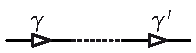
\includegraphics[scale=.8]{positiveNested}} & \raisebox{.3cm}{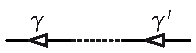
\includegraphics[scale=.8]{negativeNested}} & 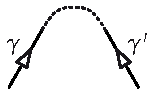
\includegraphics[scale=.8]{negativeDisjoint} & 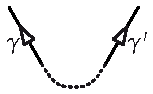
\includegraphics[scale=.8]{positiveDisjoint} \\[.2cm]
          $\so[\gamma] \subseteq \so[\gamma']$ & $\so[\gamma] \supseteq \so[\gamma']$ & $\so[\gamma] \negDisjoint \so[\gamma']$ & $\so[\gamma] \posDisjoint \so[\gamma']$
        \end{tabular}
      }
      \caption{The relative position of two arcs~$\gamma$ and~$\gamma'$ in a signed spine~$\spine$ determines the compatibility relation between their source label sets~$\so[\gamma]$ and~$\so[\gamma]$.}
      \label{fig:sourceSetsCompatible}
    \end{figure}
  \end{itemize}

  \para{Injective}
  To see the injectivity of~$\spineToNested$, we prove that we can reconstruct a spine~$\spine$ from the source sets of its arcs.
  First the the nodes of~$\spine$ are the equivalence classes under the relation~$v \equiv w$ if there is no arc~$\gamma$ of~$\spine$ such that~$|\{v,w\} \cap \so[\gamma]| = 1$.
  Second, the leaves of~$\spine$ correspond to the source sets containing either only one or all but one node of~$\spine$. 
  We can then delete one leaf~$\ell$ of~$\spine$, and reconstruct by induction the tree~$\spine \ssm \{\ell\}$. 
  Finally the only possible node of~$\spine \ssm \{\ell\}$ to which the leaf~$\ell$ can be glued is the unique node which is in the intersection of all source sets~$B$ of~$\spine \ssm \{\ell\}$ such that~$B \cup \ell$ is a source set of~$\spine$, but not in the union of all source sets~$B$ of~$\spine \ssm \{\ell\}$ such that~$B \cup \ell$ is not a source set of~$\spine$.

  \para{Surjective}
  To see the surjectivity of~$\spineToNested$, we prove that for any nested set~$\nested$ on~$\b{G}$,
\begin{enumerate}[(a)]
\item there exists a spine~$\spine$ on~$\b{G}$ such that~$\spineToNested(\spine) = \nested$, and
\item for any block~$B$ of~$\b{G}$ compatible with all blocks of~$\nested$, there exists a node~$X$ of~$\spine$ such that the partition~$X = (X \cap B) \sqcup (X \ssm B)$ is splittable (see \cref{def:splittable}).
\end{enumerate}
  These properties are proved by induction on the size of~$\nested$.  
  To initialize, observe that the rank~$0$ spine (with a single node~$\vertexSet$) is sent to the empty nested set for which Property~(b) above holds by \cref{def:block}.

  Assume now that these properties hold for a given nested set~$\nested$ and consider a bigger nested set~$\nested' \eqdef \nested \cup \{B\}$.
  Let~$\spine$ be the spine such that~$\spineToNested(\spine) = \nested$ and let~$X$ be a node of~$\spine$ such that the partition~$X = (X \cap B) \sqcup (X \ssm B)$ is splittable.
  Let~$\spine'$ denote the spine obtained by the splitting of~$(X \cap B) \sqcup (X \ssm B)$ in~$\spine$.
  We claim that $\spine$ satisfies Properties (a) and (b) above.
  
  Consider first an incoming arc~$\alpha$ of~$X$ in~$\spine$.
  Since~$B$ is compatible with~$\so[\alpha]$, and both~$X \cap B$ and~$X \ssm B$ are non-empty, we obtain that~$\so[\alpha] \subseteq B$ or~$\so[\alpha] \negDisjoint B$.
  Moreover, by \cref{def:nodeSplitting}, the arc~$\alpha$ is connected to the node~$X \cap B$ of~$\spine'$ if~$\so[\alpha] \subseteq B$, and to the node~$X \ssm B$ of~$\spine'$ if~$\so[\alpha] \negDisjoint B$.
  Similarly, for any outgoing arc~$\beta$ of~$X$ in~$\spine$, we have~$\so[\beta] \supseteq B$ or~$\so[\alpha] \posDisjoint B$, and the arc~$\beta$ is connected to the node~$X \ssm B$ of~$\spine'$ if~$\so[\beta] \supseteq B$, and to the node~$X \cap B$ of~$\spine'$ if~$\so[\beta] \posDisjoint B$.
  In particular, we have~$\so[\alpha] \subseteq B$ for each incoming arc~$\alpha$ of~$X \cap B$ in~$\spine'$, and~$\ta[\beta] \subseteq B$ for each outgoing arc~$\beta$ of~$X \cap B$ in~$\spine'$ (since~$\so[\beta] \posDisjoint B$ implies $\so[\beta] \cup B = \vertexSet$ hence $\ta[\beta] = \vertexSet \ssm \so[\beta] \subseteq B$).
  We thus obtain that~$\so[\gamma] \subseteq B$, and similarly that~$\ta[\gamma] \subseteq \vertexSet \ssm B$, from which we conclude that $\so[\gamma] = B$.
  Since~$\spine'$ is obtained by splitting a node of~$\spine$ into an arc~$\gamma$, we have~$\spineToNested(\spine') = \spineToNested(\spine) \cup \{\so[\gamma]\} = N \cup \{B\} = N '$.

  Consider now another block~$B'$ of~$\b{G}$ compatible with all blocks of~$N'$.
  Since~$B'$ is compatible with~$N \subseteq N'$, there is a node~$X'$ of~$\spine$ such that the partition~$X' = (X' \cap B') \sqcup (X' \ssm B')$ is splittable.
  If~$X \ne X'$, then~$X'$ is still a node of~$\spine'$ so that there is nothing to prove.
  If~$X = X'$, then the node~$X \cap B$ of~$\spine'$ suits if~$B \supseteq B'$ or~$B \negDisjoint B'$, while the node~$X \ssm B$ of~$\spine'$  suits if~$B \subseteq B'$ or~$B \posDisjoint B'$.
  \vincent{Check that, maybe add a sentence...}

  \para{Order-preserving}
  Finally, $\spineToNested$ is clearly order preserving as contracting one arc of a spine~$\spine$ removes the corresponding block of the nested set~$\spineToNested(\spine)$.
\end{proof}

\begin{remark}
  \label{rem:nestedToSpine}
  From the proof of \cref{prop:spineToNested}, we can give a direct description of the inverse map~$\nestedToSpine$ of the map~$\spineToNested$.
  Namely, consider a nested set~$N$ and two blocks~$B, B'$ of~$N$, and let~$\gamma, \gamma'$ denote the arcs of~$\spine \eqdef \nestedToSpine(N)$ such that~$\so[\gamma] = B$ and~$\so[\gamma'] = B'$.
  Then
  \begin{enumerate}[(i)]
    \item the target of~$\gamma$ and the source of~$\gamma'$ coincide iff~$B \subseteq B'$ and~$\nexists \, B'' \in \nested$ with~$B \subseteq B'' \subseteq B'$ or~$B \negDisjoint B'' \posDisjoint B'$,
    \item the targets of~$\gamma$ and~$\gamma'$ coincide iff~$B \negDisjoint B'$ and~$\nexists \, B'' \in \nested$ with~$B \subseteq B'' \negDisjoint B'$ or~${B \negDisjoint B'' \supseteq B'}$,
\item the sources of~$\gamma$ and~$\gamma'$ coincide iff~$B \posDisjoint B'$ and~$\nexists \, B'' \in \nested$ with~$B \posDisjoint B'' \subseteq B'$ or~${B \supseteq B'' \posDisjoint B'}$.
\end{enumerate}
This gives a description of the nodes of the spine~$\nestedToSpine(\nested)$ in terms of equivalence classes of blocks of~$\nested$ (by the relations above). It also gives a direct definition of the directed graph underlying~$\nestedToSpine(\nested)$ as a quotient of a collection of disjoint arcs labeled by~$\nested$ by identification of some of their endpoints. Finally, each node of~$\nestedToSpine(\nested)$ with incoming arcs~$A$ and outgoing arcs~$B$ is given by
\[
\bigg( \bigcap_{\beta \in B} \so[\beta] \bigg) \ssm \bigg( \bigcup_{\alpha \in A} \so[\alpha] \bigg) = \vertexSet \ssm \bigg( \bigcup_{\alpha \in A} \so[\alpha] \cup \bigcup_{\beta \in B} \ta[\beta] \bigg).
\]
\end{remark}

\begin{corollary}
  The nested complex~$\nestedComplex$ is a pure and flag simplicial complex.
\end{corollary}

%%%%%%%%%%%%%%%%%%%%%%%%%%%%%%%%%%%%%%%

\subsection{Flips}
\label{subsec:flips}

In this section, we introduce an elementary local operation on spines on~$\b{G}$.

\begin{definition}
  \label{def:flip}
  Let $\b{G}$ be a decorated block graph and let $\spine$ be a maximal spine on~$\b{G}$.
  Consider two vertices $X = \{x\}$ and $Y = \{y\}$ of $\spine$ related by an arc $\gamma$. 
  Let $\alpha$ be the incoming arc of $X$ such that~$\so[\alpha]$ and~$Y$ are contained in the same connected component of $G \ssm \Down[X]$, and let $\beta$ be the outgoing arc of $Y$ such that~$\ta[\beta]$ and~$X$ are contained in the same connected component of $G \ssm \Up[Y]$.
  We define $\spine'$ to be the spine obtained from $\spine$ by reversing the orientation of~$\gamma$, grafting the arc~$\alpha$ to~$Y$ and the arc~$\beta$ to~$X$.
  We say that $\spine'$ is obtained from $\spine$ by \defn{flipping} the arc~$\gamma$. 
\end{definition}

\begin{figure}[h!]
\centerline{
\begin{tikzpicture}[scale=1.6]  
  \node (N0) at (-0.5,-0.5) {\small $y$};
  \node (N1) at (0.5,0.5) {\small $y$};
  %
  \node (o1) at (-1.2,0.6) {\small $\beta_1$};
  \node (od) at (-0.8,0.6) {\small $\dots$};
  \node (oj) at (-0.3,0.6) {\small $\beta_k$};
  %
  \node (oj1) at (0,1.62) {\small $\beta_{k+1}$};
  \node (ojd) at (0.5,1.6) {\small $\dots$};
  \node (ol) at (1,1.6) {\small $\beta_\ell$};
  %
  \node (2) at (1.5,1.6) {\small $\boldsymbol{\beta}$};
  %
  \node (1) at (-1.5,-1.6) {\small $\boldsymbol{\alpha}$};
  %
  \node (i1) at (-1,-1.6) {\small $\alpha_1$};
  \node (id) at (-0.5,-1.6) {\small $\dots$};
  \node (im) at (0,-1.6) {\small $\alpha_i$};
  %
  \node (im1) at (0.3,-0.62) {\small $\alpha_{i+1}$};
  \node (imd) at (0.8,-0.6) {\small $\dots$};
  \node (ik) at (1.2,-0.6) {\small $\alpha_j$};
  %
  \draw[->,thick] (1)--(N0); 
  \draw[->,thick] (N1)--(2); 
  %
  \draw[->] (N0)--(o1); 
  \draw[->] (N0)--(od);
  \draw[->] (N0)--(oj);
  %  
  \draw[->] (N0)--(N1) node[midway, left] {$\gamma$} ; 
  \draw[->] (N1)--(oj1); 
  \draw[->] (N1)--(ojd);
  \draw[->] (N1)--(ol);
  %
  \draw[->] (i1)--(N0);
  \draw[->] (id)--(N0);
  \draw[->] (im)--(N0); 
  %
  \draw[->] (im1)--(N1); 
  \draw[->] (imd)--(N1);
  \draw[->] (ik)--(N1);
  \end{tikzpicture}
  \raisebox{6.5em}{
  \begin{tikzpicture}[scale=1.2]
    \draw[->] (0,0)--(1,0); 
  \end{tikzpicture}}
  \quad
  \begin{tikzpicture}[scale=1.6]  
    \node (N0) at (-0.5,0.5) {\small $x$};
    \node (N1) at (0.5,-0.5) {\small $y$};
    %  
    \node (o1) at (-1,1.6) {\small $\beta_1$};
    \node (od) at (-0.5,1.6) {\small $\dots$};
    \node (oj) at (0,1.6) {\small $\beta_k$};
    %  
    \node (oj1) at (0.3,0.62) {\small $\beta_{k+1}$};
    \node (ojd) at (0.8,0.6) {\small $\dots$};
    \node (ol) at (1.2,0.6) {\small $\beta_\ell$};
    %
    \node (i1) at (-1.2,-0.6) {\small $\alpha_1$};
    \node (id) at (-0.8,-0.6) {\small $\dots$};
    \node (im) at (-0.3,-0.6) {\small $\alpha_i$};
    %  
    \node (im1) at (0,-1.62) {\small $\alpha_{i+1}$};
    \node (imd) at (0.5,-1.6) {\small $\dots$};
    \node (ik) at (1,-1.6) {\small $\alpha_j$};
    %
    \node (2) at (-1.5,1.6) {\small $\boldsymbol{\beta}$};
    %
    \node (1) at (1.5,-1.6) {\small $\boldsymbol{\alpha}$};
    %
    \draw[->,thick] (1)--(N1); 
    \draw[->,thick] (N0)--(2); 
    %  
    \draw[->] (N0)--(o1); 
    \draw[->] (N0)--(od);
    \draw[->] (N0)--(oj);
    %    
    \draw[->] (N1)--(N0) node[midway, right] {$\gamma$} ; 
    \draw[->] (N1)--(oj1); 
    \draw[->] (N1)--(ojd);
    \draw[->] (N1)--(ol);
    %  
    \draw[->] (i1)--(N0);
    \draw[->] (id)--(N0);
    \draw[->] (im)--(N0); 
    %  
    \draw[->] (im1)--(N1); 
    \draw[->] (imd)--(N1);
    \draw[->] (ik)--(N1);
  \end{tikzpicture}
  }
  \caption{A spine flip.}
  \label{fig:generalFlip}
\end{figure}

The fact that $\spine'$ is indeed a spine is immediate from the definitions. Contracting $\gamma$ in either $\spine$ or $\spine'$, we obtain the same spine $\spine''$. 

\begin{figure}[h!]
  \resizebox{0.6\linewidth}{!}{
  \begin{tikzpicture}[circle, draw=none, minimum size=4mm, inner sep=0.1mm]  
  \node (2) at (-0.5, -0.5) {$\blue \updown[2]$};
  \node (5) at (0, 0.5) {$\blue \up[5]$};
  \node (14) at (-0.5, 1.5) {$\blue 14$};
  \node (6) at (0.5, 1.5) {$\blue 6$};
  \node (9) at (1, 2.5) {$\blue \up[9]$};
  \node (7) at (-1, -1.5) {$\blue \down[7]$};
  \node (8) at (-1.5, -2.5) {$\blue 8$};
  \node (3) at (0, -1.5) {$\blue 3$};
  %
  \draw[->] (8)--(7); 
  \draw[->] (7)--(2); 
  \draw[->] (3)--(2); 
  \draw[->] (2)--(5) node[midway, left] {$\gamma$}; 
  \draw[->] (5)--(14); 
  \draw[->] (5)--(6); 
  \draw[->] (6)--(9); 
  \end{tikzpicture}
  
  \raisebox{6.5em}{
  \begin{tikzpicture}[scale=1.2]
    \draw[->] (0,0)--(1,0); 
  \end{tikzpicture}}
  
  \begin{tikzpicture}[circle, draw=none, minimum size=4mm, inner sep=0.1mm]  
  \node (2) at (-0.5, 0.5) {$\blue \updown[2]$};
  \node (5) at (0, -0.5) {$\blue \up[5]$};
  \node (14) at (0.5, 0.5) {$\blue 14$};
  \node (6) at (-1, 1.5) {$\blue 6$};
  \node (9) at (-1.5, 2.5) {$\blue \up[9]$};
  \node (7) at (0.5, -1.5) {$\blue \down[7]$};
  \node (8) at (1, -2.5) {$\blue 8$};
  \node (3) at (-1, -0.5) {$\blue 3$};
  %
  \draw[->] (8)--(7); 
  \draw[->] (7)--(5); 
  \draw[->] (3)--(2); 
  \draw[->] (5)--(2) node[midway, right] {$\gamma$};  
  \draw[->] (5)--(14); 
  \draw[->] (2)--(6); 
  \draw[->] (6)--(9); 
  \end{tikzpicture}
  }
  \caption{Two maximal spines on the block graph of \cref{fig:mapleBlock}, related by a flip.}
  \label{fig:exampleFlip}
  \end{figure} 

\begin{lemma} 
  \label{lemma:coveringpair} 
  The spines~$\spine$ and $\spine'$ are the only spines covering $\spine''$ in the spine poset~$\spinePoset$.
\end{lemma}

\begin{proof}
  This follows from \cref{prop:nodeSplitting,prop:contractionSplitting}.
  \vincent{I don't understand why it is so simple compared to the proof in my paper...}
\end{proof}
  
\begin{definition}
  \label{def:flipGraph}
  The \defn{flip graph} is the graph whose vertices are the maximal spines on~$\b{G}$ and whose egdes are the flips between them.
  In other words, it is the facet-ridge graph of the nested complex~$\nestedComplex$.
\end{definition}

\begin{corollary} 
   The nested complex~$\nestedComplex$ is a closed pseudo-manifold. 
\end{corollary}
  
\begin{definition}
  \label{def:increasingFlip}
  Fix a total order~$\prec$ on~$\vertexSet$.
  The flip from~$\spine$ to~$\spine'$ in \cref{def:flip} is \defn{$\prec$-incresing} if~$x \prec y$ and \defn{$\prec$-decreasing} if $x \succ y$.
  The \defn{$\prec$-increasing flip graph} is the directed graph whose vertices are the maximal spines on~$\b{G}$ and whose arcs are the increasing flips between them.
  The \defn{$\prec$-increasing flip poset} is the transitive closure of the $\prec$-increasing flip graph.
\end{definition}

For instance, the flip of \cref{fig:exampleFlip} is increasing with respect to the natural order on $V$.

\begin{example}
  \label{exm:flipPosets}
  For instance, the increasing flip poset is (isomorphic to):
  \begin{enumerate}[(i)]
    \item the \defn{weak order} on permutations of~$\vertexSet$ when $\b{G}$ is complete or undecorated.
    \item the \defn{flip poset on maximal tubings} of~$G$ studied in~\cite{BarnardMcConville} when~$\b{G}$ is down decorated (in particular the classical \defn{Tamari lattice}~\cite{Tamari, HuangTamari} when~$\b{G}$ is a down decorated path).
    \item the \defn{acyclic reorientation lattice} of~$G$~\cite{Pilaud-acyclicReorientationLattices} when~$\b{G}$ is fully decorated (in particular the \defn{boolean lattice} when~$\b{G}$ is a fully decorated tree).
    \item the various \defn{permutree lattices} of~\cite{PilaudPons-permutrees} when~$G$ is a path (in particular the various type~$A$ \defn{Cambrian lattices}~\cite{Reading-CambrianLattices} for up-down decorated paths).
  \end{enumerate}
\end{example}

\begin{remark}
  The question of whether or not the increasing flip poset is a lattice is a difficult question. It depends on the decoration $\decoration$. We know that if $G$ is a path, it is always the case \cite{PilaudPons-permutrees}, for $G$ a block graph it is generally not true. See \cite{BarnardMcConville}. \guillaume{Nos calculs?; donner un exemple, un contre-exemple}\vincent{improve this remark.}
\end{remark}

%%%%%%%%%%%%%%%%%%%%%%%%%%%%%%%%%%%%%%%

\subsection{Labeled spines and blossoming spines}
\label{subsec:blossomingSpines}

For later purposes, we now add further information to a spine on~$\b{G}$.
Here, we need to manipulate both the vertices and the cliques of~$G$, thus we consider a maple tree~$M$ corresponding to the block graph~$G$.

\begin{definition}
  \label{def:labeledSpine}
  Let~$\b{M} \eqdef (M, \decoration)$ be a decorated maple tree and~$\b{G} \eqdef (G, \decoration)$ be the decorated block graph obtained by tapping~$M$.
  In a spine~$\spine$ on~$\b{G}$, we label
  \begin{itemize}
    \item each node~$X$ by the connected component~$\labeling(X)$ of~$M \ssm \big( \Up[{\so[X]}] \cup \Down[{\ta[X]}] \big)$ containing~$X$,
%    \item each arc~$\gamma$ by the intersection~$\labeling(\gamma)$ of the connected component of~$M \ssm \Up[{\so[\gamma]}]$ containing~$\ta[\gamma]$ with the connected component of~$M \ssm \Down[{\ta[\gamma]}]$ containing~$\so[\gamma]$.
    \item each arc~$\gamma$ by the connected component~$\labeling(\gamma)$ of~$M \ssm \big( \Up[{\so[\gamma]}] \cup \Down[{\ta[\gamma]}] \big)$ containing the red vertices of~$M$ adjacent to both~$\so[\gamma]$ and~$\ta[\gamma]$. \guillaume{ce ne sont pas tous les sommets de $M$?}
  \end{itemize}
  We say that the spine~$\spine$ with its labeling~$\labeling$ is a \defn{labeled spine}.
\end{definition}

\begin{figure}[h!]
\resizebox{0.8\linewidth}{!}{
\begin{tikzpicture}[circle, draw=none, minimum size=4mm, inner sep=0.1mm] 

\node (256) at (0,0) {$\blue \updown[2] \up[5] 6$};
\node (14) at (-1, 2) {$\blue 1 4$};
\node (9) at (1, 2) {$\blue \up[9]$};
\node (78) at (-1, -2) {$\blue \down[7] 8$};
\node (3) at (1, -2) {$\blue 3$};

\draw[->] (256)--(14) node[midway, left] {$ade$}; 
\draw[->] (256)--(9) node[midway, right] {$fgjk$}; 
\draw[->] (78)--(256) node[midway, left] {$adefghijk$}; 
\draw[->] (3)--(256) node[midway, right] {$bc$}; 

\end{tikzpicture}

\qquad

\begin{tikzpicture}[circle, draw=none, minimum size=4mm, inner sep=0.1mm]  
\node (2) at (-0.5, -0.5) {$\blue \updown[2]$};
\node (5) at (0, 0.5) {$\blue \up[5]$};
\node (14) at (-0.5, 1.5) {$\blue 14$};
\node (6) at (0.5, 1.5) {$\blue 6$};
\node (9) at (1, 2.5) {$\blue \up[9]$};
\node (7) at (-1, -1.5) {$\blue \down[7]$};
\node (8) at (-1.5, -2.5) {$\blue 8$};
\node (3) at (0, -1.5) {$\blue 3$};
%
\draw[->] (8)--(7) node[midway, left] {\small $adefghjk$}; 
\draw[->] (7)--(2) node[midway, left] {\small $adefghijk$}; 
\draw[->] (3)--(2) node[midway, right] {\small $bc$}; 
\draw[->] (2)--(5) node[midway, left] {\small $adefghijk$}; 
\draw[->] (5)--(14) node[midway, left] {\small $ade$}; 
\draw[->] (5)--(6) node[midway, right] {\small $fgjk$}; 
\draw[->] (6)--(9) node[midway, right] {\small $fgjk$}; 
\end{tikzpicture}
}
\caption{The labeled versions of the two spines of \cref{fig:exampleSpine}.}
\label{fig:exampleLabeledSpine}
\end{figure} 

\begin{remark}
  \label{rem:labeledSpine1}
  By definition, the labels of \cref{def:labeledSpine} are some maple subtrees of~$M$.
  Note that a maple subtree of~$M$ is completely determined by its leaves, hence by its red vertices.
  We thus simplify all pictures of labeled spines by writing only the red (letters) vertices of each label.
  \vincent{We could even just write the leaves...}
\end{remark}

\begin{remark}
  \label{rem:labeledSpine2}
  The labeling~$\labeling$ of \cref{def:labeledSpine} can be described alternatively using \cref{coro:splittablePartitions}.
  For any arc~$\gamma$ in a spine~$\spine$, denote by~$C_\gamma$ the connected component of~$M \ssm \Up[{\so[\gamma]}]$ containing~$\ta[\gamma]$ and by~$C^\gamma$ the connected component of~$M \ssm \Down[{\ta[\gamma]}]$ containing~$\so[\gamma]$.
%  For any arc~$\gamma$ in a spine~$\spine$, denote by~$C_\gamma$ (resp.~$C^\gamma$) the connected component of~$M \ssm \Up[{\so[\gamma]}]$ (resp.~$M \ssm \Down[{\ta[\gamma]}]$) containing~$\ta[\gamma]$ (resp.~$\so[\gamma]$).
  Then 
  \begin{itemize}
    \item $\labeling(X) = \bigcap_\alpha C_\alpha \; \cap \; \bigcap_\beta C^\beta$ where $\alpha$ (resp.~$\beta$) runs over incoming (resp.~outgoing) arcs~of~$X$,
    \item $\labeling(\gamma) = C_\gamma \cap C^\gamma$.
  \end{itemize}     
\end{remark}

\begin{lemma}
  \label{lem:labeledSpine}
%  We have~$\labeling(\alpha) \cap \labeling(\alpha') = \varnothing$ for two incoming arcs~$\alpha, \alpha'$ at the same node~$X$ of~$\spine$.
  We have~$\labeling(\gamma) \cap \labeling(\gamma') = \varnothing$ for any two distinct arcs~$\gamma, \gamma'$ incoming at (resp.~outgoing from) the same node of~$\spine$.
\end{lemma}

\begin{proof}
  Assume for instance that~$\alpha, \alpha'$ are distinct incoming arcs at a node~$X$ of~$\spine$.
  By \cref{def:spine}, the source sets~$\so[\alpha]$ and~$\so[\alpha']$ belong to distinct connected components~$C$ and~$C'$ of~$M \ssm \Down[X]$.
  Moreover, $\labeling(\alpha) \subseteq C$ since~$X \subseteq \ta[\alpha]$ and similarly~$\labeling(\alpha') \subseteq C'$.
  Hence~$\labeling(\alpha) \cap \labeling(\alpha') = \varnothing$.
\end{proof}

We now add a little more to a labeled spine.
This is not strictly needed for the purposes of the next section, but it enlightens the picture and will simplify some proofs in later sections.
\vincent{also needed for the operad part...}

\begin{definition}
  \label{def:blossomingTree}
  A \defn{directed blossoming tree} is a directed tree~$\spine$ with some additional 
  \begin{itemize}
    \item \defn{incoming blossoms} (arcs joining an empty node to a normal node) and 
    \item \defn{outgoing blossoms} (arcs joining a normal node to an empty node).
  \end{itemize}
  A \defn{cut} of a directed blossoming tree~$\spine$ is a set~$\Gamma$ of nodes, arcs and blossoms of~$\spine$ such that any directed path joining the source of an incoming blossom of~$\spine$ to the target of an outgoing blossom of~$\spine$ contains precisely one element of~$\Gamma$.
  When the nodes of~$\spine$ are sets, the \defn{source set}~$\so[\Gamma]$ (resp.~\defn{target set}~$\ta[\Gamma]$) of~$\Gamma$ is the union of the nodes of all connected components of~$\spine \ssm \Gamma$ which contain the source (resp.~target) of an incoming blossom.
  For instance, the set of incoming (resp.~outgoing) blossoms is a cut of~$\spine$ whose source (resp.~target) set is empty and whose target (resp.~source) set is the union of the nodes of~$\spine$.
\end{definition}

\begin{definition}
  \label{def:blossomingSpine}
  Let~$\b{M} \eqdef (M, \decoration)$ be a decorated maple tree, let~$\b{G} \eqdef (G, \decoration)$ be the decorated block graph obtained by tapping~$M$, and let~$\spine$ be a spine on~$\b{G}$.
  The \defn{blossoming spine}~$\spine\blossom$ is the labeled blossoming tree obtained from the labeled spine~$\spine$ by a adding at each node~$X$ of~$\spine$ an incoming (resp.~outgoing) blossom labeled by~$C$ for each connected component~$C$ of~$M \ssm \Down[\vertexSet]$ (resp.~of~$M \ssm \Up[\vertexSet]$) adjacent to~$X$ such that there is no incoming arc~$\alpha$ (resp.~outgoing arc~$\beta$) of~$X$ with~$\so[\alpha]$ (resp.~$\ta[\beta]$) contained in~$C$.
\end{definition}

\begin{figure}[h!]
\resizebox{0.8\linewidth}{!}{
\begin{tikzpicture}[circle, draw=none, minimum size=4mm, inner sep=0.1mm] 

\node (256) at (0,0) {$\blue \updown[2] \up[5] 6$};
\node (14) at (-1, 2) {$\blue 1 4$};
\node (9) at (1, 2) {$\blue \up[9]$};
\node (78) at (-1, -2) {$\blue \down[7] 8$};
\node (3) at (1, -2) {$\blue 3$};
\node (i) at (-1.5, -3) {};
\node (adefghjk) at (-0.5, -3) {};
\node (bc) at (1.5, -3) {};
\node (k) at (1.5, 3) {};
\node (fgj) at (0.5, 3) {};
\node (ade) at (-1.5, 3) {};
\node (bc') at (-1.5, 0.75) {};
\node (hi) at (1.5, 0.75) {};

\draw[->] (256)--(14) node[midway, left] {$ade$}; 
\draw[->] (256)--(9) node[midway, right] {$fgjk$}; 
\draw[->] (78)--(256) node[midway, left] {$adefghijk$}; 
\draw[->] (3)--(256) node[midway, right] {$bc$}; 
\draw[->] (i)--(78) node[midway, left] {$i$}; 
\draw[->] (adefghjk)--(78) node[midway, right] {$adefghjk$};
\draw[->] (bc)--(3) node[midway, right] {$bc$}; 
\draw[->] (9)--(k) node[midway, right] {$k$}; 
\draw[->] (9)--(fgj) node[midway, left] {$fgj$};
\draw[->] (14)--(ade) node[midway, left] {$ade$};
\draw[->] (256)--(bc') node[midway, left] {$bc$};
\draw[->] (256)--(hi) node[midway, right] {$hi$};

\end{tikzpicture}

\qquad

\begin{tikzpicture}[circle, draw=none, minimum size=4mm, inner sep=0.1mm]  
\node (2) at (-0.5, -0.5) {$\blue \updown[2]$};
\node (5) at (0, 0.5) {$\blue \up[5]$};
\node (14) at (-0.5, 1.5) {$\blue 14$};
\node (6) at (0.5, 1.5) {$\blue 6$};
\node (9) at (1, 2.5) {$\blue \up[9]$};
\node (7) at (-1, -1.5) {$\blue \down[7]$};
\node (8) at (-1.5, -2.5) {$\blue 8$};
\node (3) at (0, -1.5) {$\blue 3$};
\node (ade) at (-1, 2.5) {};
\node (fgj) at (0.5, 3.5) {};
\node (k) at (1.5, 3.5) {};
\node (adefghjk) at (-2, -3.5) {};
\node (i) at (-0.5, -2.5) {};
\node (bc) at (0.5, -2.5) {};
\node (bc') at (-1, 0.5) {};
\node (hi) at (1.5, 1) {};
%
\draw[->] (8)--(7) node[midway, left] {\small $adefghjk$}; 
\draw[->] (7)--(2) node[midway, left] {\small $adefghijk$}; 
\draw[->] (3)--(2) node[midway, right] {\small $bc$}; 
\draw[->] (2)--(5) node[midway, right] {\small $adefghijk$}; 
\draw[->] (5)--(14) node[midway, left] {\small $ade$}; 
\draw[->] (5)--(6) node[midway, right] {\small $fgjk$}; 
\draw[->] (6)--(9) node[midway, right] {\small $fgjk$}; 
\draw[->] (14)--(ade) node[midway, left] {\small $ade$}; 
\draw[->] (9)--(fgj) node[midway, left] {\small $fgj$}; 
\draw[->] (9)--(k) node[midway, right] {\small $k$}; 
\draw[->] (adefghjk)--(8) node[midway, left] {\small $adefghjk$}; 
\draw[->] (i)--(7) node[midway, right] {\small $i$}; 
\draw[->] (bc)--(3) node[midway, right] {\small $bc$};
\draw[->] (2)--(bc') node[midway, left] {\small $bc$};
\draw[->] (5)--(hi) node[midway, right] {\small $hi$};
\end{tikzpicture}
}
\caption{The blossoming versions of the two spines of \cref{fig:exampleSpine}.}
\label{fig:exampleBlossomingSpine}
\end{figure}

\begin{proposition}
  \label{prop:blossomingSpine}
  Let~$\b{M} \eqdef (M, \decoration)$ be a decorated maple tree, let~$\b{G} \eqdef (G, \decoration)$ be the decorated block graph obtained by tapping~$M$, and let~$\spine$ be a spine on~$\b{G}$.
  For any cut~$\Gamma$ of~$\spine\blossom$, the labels of the nodes, arcs and blossoms of~$\Gamma$ are precisely the connected components of~$M \ssm \big( \Up[{\so[\Gamma]}] \cup \Down[{\ta[\Gamma]}] \big)$.
\end{proposition}

\begin{proof}
  We prove the result by sweeping the blossoming spine~$\spine\blossom$.

  The base case is the cut~$\Gamma_\circ$ of~$\spine\blossom$ consisting of all its incoming blossoms, which are labeled by the connected components of~$M \ssm \Down[\vertexSet]$.
  Indeed, the label of any incoming blossom is a connected component of~$M \ssm \Down[\vertexSet]$ by definition.
  Conversely, for any connected component~$C$ of~$M \ssm \Down[\vertexSet]$, the set of nodes of~$\spine$ adjacent to~$C$ forms a chain in~$\spine$ by \cref{def:spine}, and~$C$ appears as an incoming blossom of the minimal node of~$\spine$ in this chain.
  
  Consider now a node~$X$ of~$\spine\blossom$, and let~$A$ denote its set of incoming arcs and blossoms.
  Consider now two cuts~$\Gamma$ and~$\Gamma'$ of~$\spine\blossom$ such that~$\Gamma \ssm A = \Gamma' \ssm \{X\}$ where~$A$ is the set of incoming arcs and blossoms of a node~$X$ of~$\spine\blossom$.
  Note that the sets~$\labeling(\alpha)$ for~$\alpha \in A$ are precisely the connected components of~$M \ssm \big( \Up[{\so[\Gamma]}] \cup \Down[{\ta[\Gamma]}] \big)$ adjacent to~$X$, and that $\labeling(X)$ is the connected component of~$M \ssm \big( \Up[{\so[\Gamma']}] \cup \Down[{\ta[\Gamma']}] \big)$ containing~$X$.
  We conclude that if the result holds for~$\Gamma$, then it also holds for~$\Gamma'$.
  The argument is symmetric for two cuts~$\Gamma$ and~$\Gamma'$ of~$\spine\blossom$ such that~$\Gamma \ssm \{X\} = \Gamma' \ssm B$ where~$B$ is the set of outgoing arcs and blossoms of a node~$X$ of~$\spine\blossom$.
  The result thus follows since any cut of~$\spine\blossom$ can be obtained from the cut~$\Gamma_\circ$ by a sequence of such moves.
\end{proof}

\begin{figure}[h!]
  \begin{tikzpicture}
    \node (0) at (0, 0) {$\updown[2] \up[5] 6$};
    \node (1) at (-3, 1) {$ade$};
    \node (2) at (-1, 1) {$hi$};
    \node (3) at (1, 1) {$fgjk$};
    \node (4) at (3, 1) {$bc$};
    \node (5) at (3, 3) {$bc$};
    \node (6) at (1.5, 3) {$k$};
    \node (7) at (0.5, 3) {$fgj$};
    \node (8) at (-1, 3) {$hi$};
    \node (9) at (-3, 3) {$ade$};
    \node (10) at (1, 2) {$\up[9]$};
    \node (11) at (-3, 2) {$14$};
    \node (12) at (-1, -1) {$adefghijk$};
    \node (13) at (1, -1) {$bc$};
    \node (14) at (-1, -2) {$\down[7] 8$};
    \node (15) at (1, -2) {$3$};
    \node (16) at (-2, -3) {$adefghjk$};
    \node (17) at (0, -3) {$i$};
    \node (18) at (1, -3) {$bc$};
    \draw[->] (18)--(15);
    \draw[->] (17)--(14);
    \draw[->] (16)--(14);
    \draw[->] (15)--(13);
    \draw[->] (14)--(12);
    \draw[->] (13)--(0);
    \draw[->] (12)--(0);
    \draw[->] (0)--(1);
    \draw[->] (0)--(2);
    \draw[->] (0)--(3);
    \draw[->] (0)--(4);
    \draw[->] (1)--(11);
    \draw[->] (2)--(8);
    \draw[->] (3)--(10);
    \draw[->] (4)--(5);
    \draw[->] (11)--(9);
    \draw[->] (10)--(7);
    \draw[->] (10)--(6);
    \draw[dotted] (-5,-3)--(16)--(17)--(18)--(5,-3);
    \draw[dashed] (-5,-2)--(14)--(15)--(5,-2);
    \draw[dotted] (-5,-1)--(12)--(13)--(5,-1);
    \draw[dashed] (-5,0)--(0)--(5,0);
    \draw[dotted] (-5,1)--(1)--(2)--(3)--(4)--(5,1);
    \draw[dashed] (-5,2)--(11)--(10)--(5,2);
    \draw[dotted] (-5,3)--(9)--(8)--(7)--(6)--(5)--(5,3);
    \node (20) at (5.5, -3) {$\down[2] \down[7]$};
    \node (21) at (5.5, -2) {$\down[2]$};
    \node (22) at (5.5, -1) {$\down[2]$};
    \node (23) at (5.5, 0) {};
    \node (24) at (5.5, 1) {$\up[2] \up[5]$};
    \node (25) at (5.5, 2) {$\up[2] \up[5]$};
    \node (26) at (5.5, 3) {$\up[2] \up[5] \up[9]$};
  \end{tikzpicture}
  \caption{A blossoming spine on the maple tree of \cref{fig:mapleBlock}, reconstructed from $\pi = 3 \down[7] 8 | \updown[2] \up[5] 6 | 149$.}
  \label{fig:blossomingSpine}
\end{figure}

%%%%%%%%%%%%%%%%%%%%%%%%%%%%%%%%%%%%%%%

\subsection{Refinement and surjection maps}
\label{subsec:surjectionMaps}

We now consider a natural refinement order on decorated block graphs and define natural surjections between the spines of refining decorated block graphs.

\begin{definition}
  \label{def:refinement}
  For two decorations~$\decoration$ and~$\decoration'$ on a set~$\vertexSet$, we say that~$\decoration$ \defn{refines}~$\decoration'$ (and that $\decoration'$ \defn{coarsens} $\decoration$) if~$\Down[\vertexSet] \subseteq \Down[\vertexSet][\decoration']$ and $\Up[\vertexSet] \subseteq \Up[\vertexSet][\decoration']$.
  For two decorated block graphs~$\b{G} \eqdef (G, \decoration)$ and~$\b{G}' \eqdef (G', \decoration')$, we say that~$\b{G}$ \defn{refines}~$\b{G}'$ (and that $\b{G}'$ \defn{coarsens} $\b{G}$) if~$G = G'$ and $\decoration$ refines~$\decoration'$.
  \vincent{picture of a pair of refining decorated block graphs, and two pairs of spines (related by the surjection, one maximal one not).}
\end{definition}

\begin{figure}
\centerline{
\begin{tikzpicture}[circle, draw=none, minimum size=4mm, inner sep=0.1mm]  
  \node (1) at (-4, -19) {$\blue 1$};
  \node (4) at (-4, -21) {$\blue 4$};
  \node (5) at (-2, -21) {$\blue \up[5]$};
  \node (7) at (-4, -23) {$\blue 7$};
  \node (8) at (0, -23) {$\blue 8$};
  \node (9) at (2, -23) {$\blue 9$};
  \node (6) at (2, -21) {$\blue 6$};
  \node (2) at (0, -19) {$\blue \updown[2]$};
  \node (3) at (2, -19) {$\blue 3$};
  %
  \draw[-] (1)--(4)--(5)--(1); 
  \draw[-] (2)--(6)--(8)--(5); 
  \draw[-] (7)--(5)--(2)--(3); 
  \draw[-] (2)--(8)--(9); 
  \draw[-] (5)--(6); 
\end{tikzpicture}
\qquad
\begin{tikzpicture}[circle, draw=none, minimum size=4mm, inner sep=0.1mm]  
\node (1) at (-4, -19) {$\blue 1$};
\node (4) at (-4, -21) {$\blue 4$};
\node (5) at (-2, -21) {$\blue \up[5]$};
\node (7) at (-4, -23) {$\blue \down[7]$};
\node (8) at (0, -23) {$\blue 8$};
\node (9) at (2, -23) {$\blue \up[9]$};
\node (6) at (2, -21) {$\blue 6$};
\node (2) at (0, -19) {$\blue \updown[2]$};
\node (3) at (2, -19) {$\blue 3$};
%
\draw[-] (1)--(4)--(5)--(1); 
\draw[-] (2)--(6)--(8)--(5); 
\draw[-] (7)--(5)--(2)--(3); 
\draw[-] (2)--(8)--(9); 
\draw[-] (5)--(6); 
\end{tikzpicture}
}
\caption{Two refining decorated block graphs: the graph on the left refines the graph on the right.}
\label{fig:refiningBlock}
\end{figure} 

\begin{figure}[h!]
\resizebox{\linewidth}{!}{
\begin{tikzpicture}[circle, draw=none, minimum size=4mm, inner sep=0.1mm] 

\node (256) at (0,0) {$\blue \updown[2] \up[5] 6$};
\node (14) at (-1, 2) {$\blue 1 4$};
\node (9) at (1, 2) {$\blue \up[9]$};
\node (78) at (-1, -2) {$\blue \down[7] 8$};
\node (3) at (1, -2) {$\blue 3$};

\draw[->] (256)--(14); 
\draw[->] (256)--(9); 
\draw[->] (78)--(256); 
\draw[->] (3)--(256); 

\end{tikzpicture}

\qquad

\begin{tikzpicture}[circle, draw=none, minimum size=4mm, inner sep=0.1mm] 

\node (256) at (0,0) {$\blue \updown[2] \up[5] 6$};
\node (14) at (-1, 2) {$\blue 1 4$};
\node (9) at (1, 2) {$\blue \up[9]$};
\node (78) at (-1, -2) {$\blue \down[7] 8$};
\node (3) at (1, -2) {$\blue 3$};

\draw[->] (256)--(14); 
\draw[->] (256)--(9); 
\draw[->] (78)--(256); 
\draw[->] (3)--(256); 

\end{tikzpicture}

\qquad

\begin{tikzpicture}[circle, draw=none, minimum size=4mm, inner sep=0.1mm]  
\node (2) at (-0.5, -0.5) {$\blue \updown[2]$};
\node (5) at (0, 0.5) {$\blue \up[5]$};
\node (14) at (-0.5, 1.5) {$\blue 14$};
\node (6) at (0.5, 1.5) {$\blue 6$};
\node (9) at (1, 2.5) {$\blue \up[9]$};
\node (7) at (-1, -1.5) {$\blue \down[7]$};
\node (8) at (-1.5, -2.5) {$\blue 8$};
\node (3) at (0, -1.5) {$\blue 3$};
%
\draw[->] (8)--(7); 
\draw[->] (7)--(2); 
\draw[->] (3)--(2); 
\draw[->] (2)--(5); 
\draw[->] (5)--(14); 
\draw[->] (5)--(6); 
\draw[->] (6)--(9); 
\end{tikzpicture}

\begin{tikzpicture}[circle, draw=none, minimum size=4mm, inner sep=0.1mm]  
\node (2) at (-0.5, -0.5) {$\blue \updown[2]$};
\node (5) at (0, 0.5) {$\blue \up[5]$};
\node (14) at (-0.5, 1.5) {$\blue 14$};
\node (6) at (0.5, 1.5) {$\blue 6$};
\node (9) at (1, 2.5) {$\blue \up[9]$};
\node (7) at (-1, -1.5) {$\blue \down[7]$};
\node (8) at (-1.5, -2.5) {$\blue 8$};
\node (3) at (0, -1.5) {$\blue 3$};
%
\draw[->] (8)--(7); 
\draw[->] (7)--(2); 
\draw[->] (3)--(2); 
\draw[->] (2)--(5); 
\draw[->] (5)--(14); 
\draw[->] (5)--(6); 
\draw[->] (6)--(9); 
\end{tikzpicture}
}
\caption{Two pairs of refining spines on the block graphs of \cref{fig:refiningBlock}. }
\label{fig:refiningSpine}
\end{figure} 

The following definition describes the natural surjection from the spines on~$\b{G}$ to the spines on~$\b{G}'$ when $\b{G}$ refines~$\b{G}'$.
It requires the labeling~$\labeling$ of the nodes and arcs of the spines described in \cref{def:labeledSpine}.

\begin{definition}
  \label{def:refinementSpines}
  Let~$M$ be a maple tree and~$G$ be the block graph obtained by tapping~$M$.
  Consider two decorations~$\decoration, \decoration'$ on~$B$ such that~$\decoration$ refines~$\decoration'$.
  To a spine~$\spine$ on~$\b{G} \eqdef (G, \decoration)$, we associate the spine~$\spine'$ on~$\b{G}' \eqdef (G, \decoration')$ obtained by contracting the empty nodes in the directed tree~$\almostSpine'$ with
  \begin{itemize}
    \item a node~$\nodeSurj{X}{D} \eqdef X \cap D$ for each node~$X$ of~$\spine$ and each connected component~$D$ of \linebreak ${M \ssm \big( \Up[{\so[X]}][\decoration'] \cup \Down[{\ta[X]}][\decoration'] \big)}$ contained in~$\labeling(X)$,
    \item an arc~$\arcSurj{\gamma}{C}$ joining the unique node~$\nodeSurj{X}{D}$ with~$C \subseteq D$ to the unique node~$\nodeSurj{Y}{E}$~with~${C \subseteq E}$ for each arc~$\gamma$ of~$\spine$ joining~$X$ to~$Y$ and each connected component~$C$ of~$M \ssm \big( \Up[{\so[\gamma]}][\decoration'] \cup \Down[{\ta[\gamma]}][\decoration'] \big)$ contained in~$\labeling(\gamma)$.
  \end{itemize}
  We denote by~$\surjectionSpines$ the map that sends the spine $\spine$ on~$\b{G}$ to the spine~$\spine'$ on~$\b{G}'$.
\end{definition}

\begin{remark}
  \label{rem:refinementBlossomingSpine}
  A similar construction sends a blossoming spine~$\spine\blossom$ on~$\b{G}$ to a blossoming spine~${\spine\blossom}'$ on~$\b{G}'$.
  Namely, we just need to add to the directed tree~$\almostSpine'$:
  \begin{itemize}
    \item an incoming (resp.~outgoing) blossom~$\arcSurj{\gamma}{C}$ attached to the unique node~$\nodeSurj{X}{D}$ with~$S \subseteq D$ for each incoming (resp.~outgoing) blossom~$\gamma$ of~$\spine\blossom$ attached to node~$X$.
  \end{itemize}
\end{remark}

Our next three statements aim at showing the correctness of \cref{def:refinementSpines}.
\vincent{Maybe first need to prove that ``unique node'' is correct.}
% For an arc~$\gamma$ of~$\spine$ joining~$X$ to~$Y$ and a connected component~$C$ of~$M \ssm \big( \Up[{\so[\gamma]}][\decoration'] \cup \Down[{\ta[\gamma]}][\decoration'] \big)$ there is a unique connected component~$D$ of ${M \ssm \big( \Up[{\so[X]}][\decoration'] \cup \Down[{\ta[X]}][\decoration'] \big)}$ containing~$C$, and a unique connected component~$E$ of ${M \ssm \big( \Up[{\so[Y]}][\decoration'] \cup \Down[{\ta[Y]}][\decoration'] \big)}$ containing~$C$. Indeed... todo.
For this, we first study the directed tree~$\almostSpine'$ described in \cref{def:refinementSpines} before contraction of the empty nodes.

\begin{lemma}
  \label{lem:refinementSpines1}
  The map~$\nodeSurj{X}{D} \mapsto X$ is a directed graph morphism from~$\almostSpine'$ to~$\spine$.
\end{lemma}

\begin{proof}
  This immediately follows from the definition, since any arc~$\arcSurj{\gamma}{C}$ joining~$\nodeSurj{X}{D}$ to~$\nodeSurj{Y}{E}$ in~$\almostSpine'$ comes from an arc~$\gamma$ joining~$X$ to~$Y$.
\end{proof}

\begin{lemma}
  \label{lem:refinementSpines2}
  For any arc~$\arcSurj{\gamma}{C}$ joining~$\nodeSurj{X}{D}$ to~$\nodeSurj{Y}{E}$ in~$\almostSpine'$, any (non-directed) path~$\pi$ in~$\almostSpine'$ containing~$\arcSurj{\gamma}{C}$, and any node~$\nodeSurj{Z}{F}$ in the connected component of~$\pi \ssm \arcSurj{\gamma}{C}$ containing~$\nodeSurj{X}{D}$ (resp.~$\nodeSurj{Y}{E}$), the set~$F$ is contained in the connected component of~$M \ssm \Down[\nodeSurj{Y}{E}]$ (resp.~of~$M \ssm \Up[\nodeSurj{X}{D}]$) containing~$C$.
\end{lemma}

\begin{proof}
  We prove this statement simultaneously on all arcs of~$\almostSpine'$, by induction on the length of~$\pi$.
  By symmetry, we only treat the case when~$\nodeSurj{Z}{F}$ is in the connected component of~$\pi \ssm \arcSurj{\gamma}{C}$ containing~$\nodeSurj{X}{D}$.
  
  We start with the base case of the induction when~$\pi$ is just the arc~$\arcSurj{\gamma}{C}$.
  Observe first that since~$\gamma$ joins~$X$ to~$Y$, the set~$Y$ is contained in both~$\ta[\gamma]$ and~$\ta[X]$.
  Since~$\nodeSurj{Y}{E} \subseteq Y$, it follows that both~$C$ and~$D$ are contained in a connected component of~$M \ssm \Down[\nodeSurj{Y}{E}]$.
  Since~$C \subseteq D$, we conclude that~$D$ is contained in the connected component of~$M \ssm \Down[\nodeSurj{Y}{E}]$ containing~$C$.
%  By symmetry, $E$ is contained in the connected component of~$M \ssm \Up[\nodeSurj{X}{D}]$ containing~$C$.
  
  Consider now an arbitrary path~$\pi$ containing~$\arcSurj{\gamma}{C}$ and a node~$\nodeSurj{Z}{F}$ in the connected component of~$\pi \ssm \arcSurj{\gamma}{C}$ containing~$\nodeSurj{X}{D}$.
%  By induction, we can assume that~$\nodeSurj{Z}{F}$ is an endpoint of~$\pi$, and we denote by~$\arcSurj{\eta}{G}$ the arc of~$\pi$ incident to~$\nodeSurj{Z}{F}$, and by~$\nodeSurj{W}{H}$ the other endpoint of~$\arcSurj{\eta}{G}$.
  We distinguish two situations:
  \begin{itemize}
    \item If~$\pi$ has a node~$\nodeSurj{W}{G}$ with two outgoing arcs in between~$\nodeSurj{Y}{E}$ and~$\nodeSurj{Z}{F}$, then the induction hypothesis ensures that~$E$ and~$F$ are contained in distinct connected components of~${M \ssm \Up[\nodeSurj{W}{G}]}$ and that~$G$ is contained in the connected component of~$M \ssm \Down[\nodeSurj{Y}{E}]$ containing~$C$. This implies that~$F$ is contained in the connected component of~$M \ssm \Down[\nodeSurj{Y}{E}]$ containing~$C$.
    \item Otherwise, the path~$\pi$ has a directed subpath from~$\nodeSurj{Z}{F}$ to~$\nodeSurj{Y}{E}$. Let~$\nodeSurj{W}{G}$ denote the node after~$\nodeSurj{Z}{F}$ and~$\arcSurj{\eta}{H}$ the arc joining~$\nodeSurj{Z}{F}$ to~$\nodeSurj{W}{G}$. By induction, $G$ is contained in the connected component of~$M \ssm \Down[\nodeSurj{Y}{E}]$ containing~$C$. Since~$\nodeSurj{Y}{E} \subseteq Y \subseteq \ta[Z]$, the set~$F$ is contained in the connected component of~$M \ssm \Down[\nodeSurj{Y}{E}]$. Since~$H$ is a subset of both~$F$ and~$G$, we thus obtain that~$F$ is contained in the connected component of~$M \ssm \Down[\nodeSurj{Y}{E}]$ containing~$C$. \qedhere
  \end{itemize}
%  We conclude by symmetry if~$\nodeSurj{Z}{F}$ in the connected component of~$\pi \ssm \arcSurj{\gamma}{C}$ containing~$\nodeSurj{Y}{F}$.
\end{proof}

\begin{lemma}
  \label{lem:refinementSpines2}
  For any spine~$\spine$ on~$\b{G}$, the graph~$\spine'$ is indeed a spine on~$\b{G}'$.
\end{lemma}

\begin{proof}
  We first prove that~$\almostSpine'$ is indeed a directed tree, by proving that it is connected and acyclic.
  \begin{itemize}
    \item \uline{connected}: Consider an edge~$\{u,v\}$ of~$G$. Since~$u$ and~$v$ belong to the same connected component of~$G \ssm U$ for any subset~$U$ of~$\vertexSet$, there is a directed path~$\pi$ in~$\spine$ between the node containing~$u$ and the node containing~$v$. For any node~$X$ (resp.~arc~$\gamma$) in the interior of this path, $u$ and~$v$ also belong to the same connected component~$D_\star$~of~$M \ssm \big( \Up[{\so[X]}][\decoration'] \cup \Down[{\ta[X]}][\decoration'] \big)$ (resp.~$C_\star$~of~$M \ssm \big( \Up[{\so[\gamma]}][\decoration'] \cup \Down[{\ta[\gamma]}][\decoration'] \big)$). The corresponding nodes~$\nodeSurj{X}{D_\star}$ and arcs~$\arcSurj{\gamma}{C_\star}$ along the path~$\pi$ thus form a path in~$\almostSpine'$ between the node containing~$u$ and the node containing~$v$. The connectedness of~$G$ thus implies the connectedness of~$\almostSpine'$.
    \item \uline{acyclic}: Assume that~$\almostSpine'$ contains a (non-directed) cycle~$\sigma'$. By \cref{lem:refinementSpines1}, the corresponding arcs in~$\spine$ also form a (non-directed, with possible edge repetitions) cycle~$\sigma$. Since~$\spine$ is a directed tree, $\sigma$ has two incoming arcs at the same node. Hence, $\sigma'$ also has two incoming arcs at the same node. Therefore, there are two paths in~$\almostSpine'$ starting at the same node and arriving to the same node through different incoming arcs, contradicting \cref{lem:refinementSpines2}.
  \end{itemize}
  We conclude that~$\spine'$ is a directed tree as it is obtained by contractions in the directed tree~$\almostSpine'$.
  We thus just need to check the two conditions of \cref{def:spine}.

  First, since any node~$X$ of~$\spine$ is contained both in~$\labeling(X)$ and in ${M \ssm \big( \Up[{\so[X]}][\decoration'] \cup \Down[{\ta[X]}][\decoration'] \big)}$, the non-empty nodes~$\nodeSurj{X}{D}$ partition the node~$X$.
  Hence, since the nodes of~$\spine$ partition~$\vertexSet$, the nodes of~$\spine'$ partition~$\vertexSet$. This shows the global condition of \cref{def:spine}.

  Finally, consider two incoming arcs~$\arcSurj{\alpha}{C}$ and~$\arcSurj{\alpha'}{C'}$ of a node~$\nodeSurj{X}{D}$ in~$\almostSpine$.
  By \cref{lem:refinementSpines2}, the source sets $\so[\arcSurj{\alpha}{C}]$ and~$\so[\arcSurj{\alpha'}{C'}]$ are contained in distinct connected components of~$G \ssm \Down[\nodeSurj{X}{D}]$.
  By symmetry, we thus conclude that~$\almostSpine'$, and thus~$\spine'$, satisfies the local condition of \cref{def:spine}.
\end{proof}

We now describe the surjection map~$\surjectionSpines$ in terms of extensions defined in \cref{def:preorderSpine} and the spine poset of \cref{def:spinePoset}.

\begin{proposition}
  \label{prop:alternativeDescriptionRefinementSpines}
%  Let~$\b{G}$ and~$\b{G}'$ be two decorated block graphs such that~$\b{G}$ refines~$\b{G'}$.
  The spine~$\surjectionSpines(\spine)$ is the unique contraction minimal spine on~$\b{G}'$ extended by the spine~$\spine$ of~$\b{G}$.
\end{proposition}

\begin{proof}
  Observe first that 
  \begin{itemize}
    \item if~$\spine$ extends~$\spine'$, then each node~$X$ of~$\spine$ is the disjoint union of nodes~$X'_1, \dots, X'_k$ of~$\spine'$.
    \item if~$\spine$ extends~$\spine'$, then~$\spine'$ is a minimal spine extended by~$\spine$ if and only if for each node~$X$ of~$\spine$ is the disjoint union of nodes~$X'_1, \dots, X'_k$ incomparable in~$\spine'$.
  \end{itemize}
  It follows that~$\surjectionSpines(\spine)$ is indeed a minimal spine on~$\b{G}'$ extended by~$\spine$.
  Moreover, the spines of~$\b{G}'$ extended by~$\spine$ form an upper ideal of the spine poset~$\spinePoset[\b{G}']$.
  We thus need to show that it is the only minimal spine on~$\b{G}'$ extended by~$\spine$.
  \vincent{todo}
\end{proof}

\begin{corollary}
  \label{coro:preimageRefinementSpines}
  For a spine~$\spine'$ on~$\b{G}'$, the preimage~$\surjectionSpines^{-1}(\spine')$ is the set of spines on~$\b{G}$ that extend~$\spine'$ but no spine on~$\b{G}'$ strictly below~$\spine'$ in~$\spinePoset[\b{G}']$.
  \vincent{Not really useful... I want to say that the map is surjective. What is the simplest way to see it?}
\end{corollary}

\begin{corollary}
  \label{coro:preimageRefinementMaximalSpines}
  For a maximal spine~$\spine'$ on~$\b{G}'$, the preimage~$\surjectionSpines^{-1}(\spine')$ is the set of maximal spines on~$\b{G}$ that extend~$\spine'$.
\end{corollary}

\begin{proposition}
  \label{prop:refinementSpines}
  If~$\b{G}$ refines~$\b{G}'$, then the map~$\surjectionSpines$ is 
  \begin{itemize}
    \item a surjection from the spines on~$\b{G}$ to the spines on~$\b{G}'$,
    \item a filtered map from the spine poset~$\spinePoset[\b{G}]$ to the spine poset~$\spinePoset[\b{G}']$, meaning that the rank of~$\surjectionSpines(\spine)$ is at least the rank of~$\spine$ (it can have more, see \cref{fig:blossomingSpine}).
  \end{itemize}
\end{proposition}

\begin{proof}
  \vincent{todo}
\end{proof}

\begin{definition}
  \label{def:equivalenceRelation}
  If~$\b{G}$ refines~$\b{G}'$, then the fibers of the surjection~$\surjectionSpines$ define an equivalence relation~$\equivalenceSpines$ on spines of~$\b{G}$. In other words, $\spine \equivalenceSpines \spine'$ if and only if~$\surjectionSpines(\spine) = \surjectionSpines(\spine')$.
\end{definition}

\begin{example}
  \label{exm:equivalenceRelations}
  \vincent{improve}
  For instance, the equivalence relation~$\equiv_\b{G}$ on permutations is
  \begin{enumerate}[(i)]
    \item the \defn{trivial relation} when $\b{G}$ is complete or undecorated.
    \item the various \defn{permutree relations} of~\cite{PilaudPons-permutrees} when~$G$ is a path (in particular the \defn{sylvester relation} for a down decorated path, and the \defn{Cambrian relations} for up-down decorated~paths).
  \end{enumerate}
  Note that in contrast to these specific examples, the equivalence relation~$\equiv$ has no reason to be a lattice congruence of the weak order.
\end{example}

\begin{proposition}
  \label{prop:equivalenceRelation}
  The equivalence relation $\equivalenceSpines$ is the transitive closure of the rewriting rule...
  \vincent{todo: rewriting rule}
\end{proposition}

We finally compare the nested complexes~$\nestedComplex[\b{G}]$ and~$\nestedComplex[\b{G}']$
\vincent{Not sure where I want that...}

\begin{proposition}
  \label{prop:refinementBlocks}
  If~$\b{G}$ refines~$\b{G}'$, then
  \begin{itemize}
    \item any block of~$\b{G}'$ is a block of~$\b{G}$,
    \item the nested complex~$\nestedComplex[\b{G}']$ contains the subcomplex of~$\nestedComplex[\b{G}]$ induced by the blocks of~$\b{G}'$.
  \end{itemize}
\end{proposition}

\begin{proof}
  \vincent{todo}
\end{proof}

%%%%%%%%%%%%%%%%%%%%%%%%%%%%%%%%%%%%%%%

\subsection{Links}
\label{subsec:links}

Finally, we describe the links of the nested complexes.
It turns out that we have a sufficiently large family of simplicial complexes so that their links are just cartesian products of simplicial complexes in this family.

\vincent{need to explain links in terms of spines as well...}

\begin{definition}
  \label{def:subBlockGraph}
  Let~$M$ be a maple tree, let~$G$ be the block graph obtained by tapping~$M$, and let~$X \sqcup Y = \vertexSet$ be a partition of the vertex set~$\vertexSet$ of~$G$ (thus of the blue vertices of~$M$).
  We denote by~$M_X$ the maple tree with blue vertices~$X$ obtained by contracting all edges of~$M$ incident to a vertex of~$Y$ (note that each red vertex of~$M_X$ is labeled by the concatenation of the labels of the corresponding red vertices in~$M$).
  We denote by~$G_X$ the block graph with vertices~$X$ obtained by replacing each connected component of~$Y$ in~$G$ by a clique on its neighbors in~$G$.
  Note that $G_X$ is obtained by tapping~$M_X$.
  For a decorated maple tree~$\b{M} \eqdef (M,\decoration)$ and a decorated block graph~$\b{G} \eqdef (G,\decoration)$, we define~$\b{M}_X \eqdef (M_X, \decoration_X)$ and~$\b{G}_X \eqdef (G_X, \decoration_X)$ where~$\decoration_X$ is the restriction of~$\decoration$ to~$X$.
\end{definition}

\begin{definition}
  \label{def:insert}
  Let~$\b{M}$ be a decorated maple tree and~$\b{G}$ be the decorated block graph obtained by tapping~$M$.
  Let~$\spine\blossom$ be a blossoming spine on~$\b{G}$, and let~$\spine\blossom_X$ be a blossoming spine on~$\b{G}_X$ for each node~$X$ of~$\spine\blossom$.
  Note that the connected components of~$M_X \ssm \Down[X]$ (resp.~of~$M_X \ssm \Up[X]$) label both the incoming (resp.~outgoing) blossoms of~$\spine\blossom_X$ and the incoming (resp.~outgoing) arcs and blossoms at~$X$ in~$\spine\blossom$.
  We denote by~$\insertion{\spine\blossom}{(\spine\blossom_X)_{X \in \spine\blossom}}$ the blossoming spine on~$\b{G}$ obtained by replacing each node~$X$ of~$\spine\blossom$ by the blossoming spine~$\spine\blossom_X$ (and reconnecting the blossoms of~$\spine\blossom_X$ to the arcs of~$\spine\blossom$ according to their labels).
  \vincent{We need a picture}
\end{definition}

\begin{lemma}
  \label{lem:insert}
  The directed tree~$\insertion{\spine\blossom}{(\spine\blossom_X)_{X \in \spine\blossom}}$ is indeed a blossoming spine on~$\b{G}$.
\end{lemma}

\begin{proof}
  \vincent{todo}
\end{proof}

\begin{proposition}
  \label{prop:linksSpines}
  The blossoming spines on~$\b{G}$ which can be contracted to a given blossoming spine~$\spine\blossom$ on~$\b{G}$ are precisely the blossoming spines~$\insertion{\spine\blossom}{(\spine\blossom_X)_{X \in \spine\blossom}}$ for all choices of a blossoming spine~$\spine\blossom_X$ on~$\b{G}_X$ for each node~$X$ of~$\spine\blossom$.
\end{proposition}

\begin{proof}
  \vincent{todo}
\end{proof}

\cref{prop:linksSpines} rephrases as follows on the spine poset of \cref{subsec:spinePoset}, on the nested complex of \cref{subsec:nestedComplex}, and on the flip graph of \cref{subsec:flips}.
\vincent{Maybe keep only the second one?}

\begin{corollary}
  \label{coro:linksSpinePoset}
  The upper ideal of the spine poset~$\spinePoset$ generated by a given spine~$\spine$ is isomorphic to the Cartesian product of the spine posets~$\spinePoset[\b{G}_X]$ for the nodes~$X$ of~$\spine$.
\end{corollary}

\begin{corollary}
  \label{coro:linksNestedComplex}
  The link of the face of the nested complex~$\nestedComplex$ corresponding to a spine~$\spine$ is isomorphic to the join of the nested complexes~$\nestedComplex[\b{G}_X]$ for the nodes~$X$ of~$\spine$.
\end{corollary}

\begin{corollary}
  \label{coro:linksFlipGraph}
  The flip graph on the maximal spines on~$\b{G}$ that contract to a spine~$\spine$ is isomorphic to the Cartesian product of the flip graphs on maximal spines of~$\b{G}_X$ for the nodes~$X$ of~$\spine$.
\end{corollary}

%%%%%%%%%%%%%%%%%%%%%%%%%%%%%%%%%%%%%%%
%%%%%%%%%%%%%%%%%%%%%%%%%%%%%%%%%%%%%%%

\section{Geometry: Spine Fans and Polytopes}
\label{sec:geometry}

We denote by~$(\b{e}_v)_{v \in \vertexSet}$ the standard basis of~$\R^{\vertexSet}$.
We denote by~$\one_X \eqdef \sum_{x \in X} \b{e}_x$ the characteristic vector of a subset~$X \subseteq \vertexSet$, and write just~$\one$ for~$\one_{\vertexSet}$.
%We consider the hyperplane
%\[
%\Hyp \eqdef \bigset{\b{x} \in \R^{\vertexSet}}{\dotprod{\one}{\b{x}} = \weight_{\vertexSet}}.
%\]

%%%%%%%%%%%%%%%%%%%%%%%%%%%%%%%%%%%%%%%

\subsection{Spine fan}
\label{subsec:spineFan}

%We first recall some observations on the braid arrangement (see \eg \cite{Postnikov, PostnikovReinerWilliams}) and on graphical arrangements.
%
Recall that a (polyhedral) \defn{cone} is the positive span of a finite set of vectors, or equivalently the intersection of a finite set of linear halfspaces.
The \defn{faces} of a cone are its intersections with its supporting linear hyperplanes.
A (polyhedral) \defn{fan}~$\c{F}$ is a collection of polyhedral cones closed under faces (if~$\polytope{C}$ is a face of~$\polytope{C'}$, then~$\polytope{C'} \in \c{F} \Rightarrow \polytope{C'} \in \c{F}$) and intersecting along faces (any two cones of~$\c{F}$ intersect along a face of both).
The \defn{rays} of~$\c{F}$ are its dimension~$1$ cones, and the \defn{regions} of~$\c{F}$ are its inclusion maximal cones.
The fan~$\c{F}$ is \defn{essential} when its inclusion minimal cone is the origin, \defn{complete} when its cones cover the space, and \defn{simplicial} when all its cones are simplicial (generated by linearly independent vectors).
In this paper, all the fans live in the hyperplane~${\Hyp[0] \eqdef \bigset{\b{x} \in \R^{\vertexSet}}{\dotprod{\one}{\b{x}} = 0}}$ of~$\R^{\vertexSet}$.

%We next consider two very classical examples of fans.
%
%\begin{example}
%  \label{exm:braidFan}
%  The \defn{braid arrangement} is the collection of hyperplanes~$\set{\b{x} \in \R^{\vertexSet}}{x_u = x_v}$ for all~$u \ne v \in \vertexSet$.
%  Since this arrangement is not essential (all its hyperplanes contain the line generated by~$\one$), we consider its intersection with the hyperplane~${\Hyp[0] \eqdef \bigset{\b{x} \in \R^{\vertexSet}}{\dotprod{\one}{\b{x}} = 0}}$.
%  This intersection defines the \defn{braid fan}~$\braidFan$.
%  Each surjection~$\pi : \vertexSet \to [k+1]$ corresponds to a $k$-dimensional cone~$\normalCone(\pi) \eqdef \set{\b{x} \in \Hyp[0]}{x_u \le x_v \text{ iff } \pi(u) \le \pi(v)}$ of~$\braidFan$.
%  In particular, the regions of~$\braidFan$ correspond to bijections~$\vertexSet \to [|\vertexSet|]$ and the rays of~$\braidFan$ correspond to proper subsets of~$\varnothing \ne X \ne \vertexSet$.
%  \vincent{Not sure if we want surjections or ordered partitions here.}
%%More generally, we associate to an acyclic oriented graph~$H$ whose nodes partition~$\vertexSet$ the cone~$\normalCone(H) \eqdef \set{\b{x} \in \Hyp[0]}{x_u \le x_v \text{ for all } u \preccurlyeq_H v}$, where~$u \preccurlyeq_H v$ means that there is a directed path in~$H$ from the node containing~$u$ to the node containing~$v$ (in particular, ~$u =_H v$ if~$u$ and~$v$ belong to the same node of~$H$).
%%Recall that a \defn{preposet} on~$\vertexSet$ is a reflexive and transitive binary relation~$R \subsetea \vertexSet \times \vertexSet$.
%%An equivalence relation is a symmetric preposet, and a poset if an antisymmetric preposet.
%%Any preposet~$R$ decomposes into an equivalence relation~$\equiv_R \eqdef \set{(u,v) \in R}{(v,u) \in R}$ together with a poset structure~${\prec_R \eqdef \, R/\!\equiv_R}$ on the equivalence classes of~$\equiv_R$.
%%Let~$H$ be an acyclic oriented graph~$H$ whose nodes partition~$\vertexSet$.
%%For two vertices~$u,v \in \vertexSet$, we write~$u \preccurlyeq_H v$ if there is a directed path in~$H$ from the node containing~$u$ to the node containing~$v$ (in particular, ~$u =_H v$ if~$u$ and~$v$ belong to the same node of~$H$).
%%We associate to~$H$ the two cones
%%\[
%%  \normalCone(H) \eqdef \set{\b{x} \in \Hyp[0]}{x_u \le x_v \text{ for all } u \preccurlyeq_H v}
%%  \quad\text{and}\quad
%%  \primalCone(H) \eqdef \cone\set{\b{e}_u - \b{e}_v}{\text{for all } u \preccurlyeq_H v}.
%%\]
%%Note that these two cones are polar to each other.
%\end{example}
%
%\vincent{We could introduce here the sylvester fan. But it would be a repetition with the spine fan. Not sure.}
%%\begin{example}
%%  \label{exm:sylvesterFan}
%%  \vincent{Todo}
%%\end{example}
%
%\begin{example}
%  \label{exm:graphicalFan}
%  The \defn{graphical arrangement} of~$G$ is the collections of hyperplanes~$\set{\b{x} \in \R^{\vertexSet}}{x_u = x_v}$ for all~$\{u,v\} \in \edgeSet$.
%  Its intersection with the hyperplane~$\Hyp[0]$ defines the \defn{graphical fan}~$\graphicalFan$.
%  The cones of~$\graphicalFan$ correspond to the pairs~$(p,o)$ where~$p$ is a partition of~$\vertexSet$ into connected subgraphs, and~$o$ is an acyclic orientation of the quotient graph~$G/p$.
%  In particular, the regions of~$\graphicalFan$ correspond to the acyclic orientations of~$G$.
%\end{example}
%
%We consider the following fan which is sandwiched between the braid fan and the graphical fan.

\begin{definition}
  \label{def:spineFan}
  For a spine~$\spine$, we denote by~$\normalCone(\spine)$ the cone of~$\Hyp[0]$ defined by the inequalities~${x_u \le x_v}$ for all~$u,v \in \vertexSet$ such that there is a directed path in~$\spine$ joining the node containing~$u$ to the node containing~$v$ in~$\spine$ (in particular, $x_u = x_v$ when $u,v \in \vertexSet$ belong to the same node of~$\spine$).
%  \[
%    \normalCone(\spine) \eqdef \set{\b{x} \in \Hyp[0]}{x_u \le x_v \text{ for all (possibly trivial) directed paths } u \to v \text{ in } \spine}
%  \]
  The \defn{spine fan}~$\spineFan$ is the collection of cones~$\normalCone(\spine)$ for all spines~$\spine$ on~$\b{G}$.  
\end{definition}

\begin{proposition}
  \label{prop:spineFan}
  The spine fan~$\spineFan$ is a complete simplicial fan on~$\Hyp[0]$.
\end{proposition}

\begin{proof}
  Since each spine~$\spine$ on~$\b{G}$ is a directed tree, the cone~$\normalCone(\spine)$ is simplicial, and its faces are the cones~$\normalCone(\spine')$ for all spines~$\spine'$ obtained by repeated arc contractions in~$\spine$ (in other words, for all spines in the lower ideal of the spine poset~$\spinePoset$ generated by~$\spine$).
  We thus just need to prove that the cones~$\normalCone(\spine)$ properly intersect and cover~$\Hyp[0]$, or equivalently, that the relative interiors of the cones~$\normalCone(\spine)$ partition~$\Hyp[0]$.
  This immediately follows from \cref{prop:alternativeDescriptionRefinementSpines}.
\end{proof}

\begin{corollary} 
   The nested complex~$\nestedComplex$ is a simplicial sphere.
\end{corollary}

%\begin{proposition}
%  \label{prop:fanSandwich}
%  The spine fan~$\spineFan$ coarsens the braid fan~$\braidFan$ and refines the graphical fan~$\graphicalFan$.
%\end{proposition}
%
%\begin{proof}
%  This immediately follows from \cref{subsec:surjectionMaps}.
%\end{proof}

%\begin{example}
%  \label{exm:braidFanGraphicalFan}
%  The spine fan~$\spineFan$ recovers the braid fan~$\braidFan$ of \cref{exm:braidFan} and the graphical fan~$\graphicalFan$ of \cref{exm:graphicalFan} in the following two extreme situations:
%  \begin{itemize}
%    \item if~$\Down[\vertexSet] = \Up[\vertexSet] = \varnothing$, then the spine fan~$\spineFan$ is the braid fan~$\braidFan$,
%    \item if~$\Down[\vertexSet] = \Up[\vertexSet] = \vertexSet$, then the spine fan~$\spineFan$ is the graphical fan~$\graphicalFan$.
%  \end{itemize}
%\end{example}

\begin{example}
  \label{exm:spineFans}
  For instance, the spine fan is:
  \begin{enumerate}[(i)]
    \item the \defn{braid fan}~$\braidFan$ when~$\b{G}$ is complete or undecorated. It is the fan defined from the classical \defn{braid arrangement} of the hyperplanes~$\set{\b{x} \in \R^{\vertexSet}}{x_u = x_v}$ for all vertices~$u \ne v \in \vertexSet$. It has a $k$-dimensional cone~$\normalCone(\pi) \eqdef \set{\b{x} \in \Hyp[0]}{x_u \le x_v \text{ iff } \pi(u) \le \pi(v)}$ for each surjection~$\pi : \vertexSet \to [k+1]$. In particular, the regions of~$\braidFan$ correspond to bijections~${\vertexSet \to [|\vertexSet|]}$ and the rays of~$\braidFan$ correspond to proper subsets of~$\varnothing \ne X \ne \vertexSet$.
    \item the \defn{nested fan} of~$G$ studied in~\cite{CarrDevadoss, Zelevinsky} when~$\b{G}$ is down decorated (in particular the classical \defn{sylvester fan} when~$\b{G}$ is a down decorated path).
    \item the \defn{graphical fan}~$\graphicalFan$ when~$\b{G}$ is fully decorated (in particular the \defn{coordinate fan} when~$\b{G}$ is a fully decorated tree). It is the fan defined from the \defn{graphical arrangement} of the hyperplanes~$\set{\b{x} \in \R^{\vertexSet}}{x_u = x_v}$ for all edges~$\{u, v\} \in \vertexSet$. The cones of~$\graphicalFan$ correspond to the pairs~$(p,o)$ where~$p$ is a partition of~$\vertexSet$ into connected subgraphs, and~$o$ is an acyclic orientation of the quotient graph~$G/p$. In particular, the regions of~$\graphicalFan$ correspond to the acyclic orientations of~$G$.
    \item the various \defn{permutree fans} of~\cite{PilaudPons-permutrees} when~$G$ is a path (in particular the various type~$A$ \defn{Cambrian fans} for up-down decorated paths).
  \end{enumerate}
\end{example}

\begin{proposition}
  \label{prop:refinementSpineFan}
  If~$\b{G}$ refines~$\b{G}'$, the spine fan~$\spineFan[\b{G}]$ refines the spine fan~$\spineFan[\b{G}']$.
  In particular, the spine fan~$\spineFan$ coarsens the braid fan~$\braidFan$ and refines the graphical fan~$\graphicalFan$.
\end{proposition}

\begin{proof}
  Follows from \cref{prop:refinementEquivalenceRelations}.
\end{proof}

%%%%%%%%%%%%%%%%%%%%%%%%%%%%%%%%%%%%%%%

\subsection{Spine polytope}
\label{subsec:spinePolytope}

Recall that a \defn{polytope}~$\polytope{P}$ is the convex hull of a finite set of points, or equivalently a bounded intersection of a finite set of affine halfspaces.
The \defn{faces} of~$\polytope{P}$ are its intersections with its supporting affine hyperplanes.
The \defn{vertices} of~$\polytope{P}$ are its dimension~$0$ faces, and the \defn{facets} of~$\polytope{P}$ are its codimension~$1$ faces.
The \defn{normal cone} of a face~$\polytope{F}$ of~$\polytope{P}$ is the cone of all linear functions whose maximum over~$\polytope{P}$ is attained precisely on~$\polytope{F}$.
The \defn{normal fan} of~$\polytope{P}$ is the fan formed by the normal cones of all the faces of~$\polytope{P}$.
All our polytopes are parametrized by a weight function, which does not change their combinatorics but provides more freedom for their geometry.

\begin{definition}
  \label{def:weight}
  For a set~$X$, we denote by~$\monombinom{X}$ the set of~$\binom{|X|+1}{2}$ subsets of~$X$ of size $1$ or~$2$.
  We fix a \defn{weight}~$\weight_p$ for all~$p \in \monombinom{\vertexSet}$, and we define~$\weight_X \eqdef \sum_{p \in \monombinom{X}} \weight_p$ for any subset~$X$ of~$\vertexSet$.
\end{definition}

%We next consider two very classical examples of polytopes.
%
%\begin{example}
%  \label{exm:permutahedron}
%  The \defn{permutahedron}~$\Perm$ is the polytope defined equivalently as
%  \begin{itemize}
%%    \item the convex hull of the points~$\sum_{u,v \in \vertexSet} \delta_{\sigma(u) \le \sigma(v)} \weight_{uv} \b{e}_v$ for all bijections~$\sigma: \vertexSet \to [|\vertexSet|]$,
%    \item the convex hull of the points~$\point[\sigma] \eqdef \sum_{p \in \monombinom{\vertexSet}} \weight_p \b{e}_{\max_\sigma(p)}$ for all bijections~$\sigma: \vertexSet \to [|\vertexSet|]$,
%    \item the intersection of the affine hyperplane~$\Hyp \eqdef \bigset{\b{x} \in \R^{\vertexSet}}{\dotprod{\one}{\b{x}} = \weight_{\vertexSet}}$ with the affine halfspaces~$\HS_X \eqdef \bigset{\b{x} \in \R^{\vertexSet}}{\dotprod{\one_X}{\b{x}} \ge \weight_X}$ for all proper subsets~$\varnothing \ne X \subsetneq \vertexSet$,
%    \item the Minkowski sum~$\sum_{p \in \monombinom{\vertexSet}} \weight_p \triangle_p$, where~$\triangle_p \eqdef \conv\set{\b{e}_v}{v \in p}$.
%  \end{itemize}
%  The braid fan~$\braidFan$ is the normal fan of the permutahedron~$\Perm$.
%  Note that the barycenter of~$\Perm$ is the point~$\b{0}^\weight \eqdef \sum_{p \in \monombinom{\vertexSet}} \frac{\weight_p}{|p|} \one_p$.
%\end{example}
%
%\vincent{We could introduce here the graph associahedron. But it would be a repetition with the spine fan. Not sure.}
%\begin{example}
%  \label{exm:associahedron}
%  The \defn{graph associahedron}~$\Asso$ is the polytope defined equivalently as
%  \vincent{todo}
%  \begin{itemize}
%    \item the convex hull of the points~$\point[{\spine[T]}] \eqdef \dots$,
%    \item the intersection of the affine hyperplane~$\Hyp \eqdef \bigset{\b{x} \in \R^{\vertexSet}}{\dotprod{\one}{\b{x}} = \weight_{\vertexSet}}$ with the affine halfspaces~$\HS_X \eqdef \bigset{\b{x} \in \R^{\vertexSet}}{\dotprod{\one_X}{\b{x}} \ge \weight_X}$ for all proper subsets~$\varnothing \ne X \subsetneq \vertexSet$ which induce a connected subgraph of~$G$,
%    \item the Minkowski sum~$\sum_{X} \weight_X \triangle_X$, where~$\triangle_X \eqdef \conv\set{\b{e}_u}{u \in X}$.
%  \end{itemize}
%  The sylvester fan~$\sylvesterFan$ is the normal fan of the associahedron~$\Asso$.
%\end{example}
%
%\begin{example}
%  \label{exm:graphicalZonotope}
%  The \defn{graphical zonotope}~$\Zono$ is the polytope defined as...
%  The graphical fan~$\graphicalFan$ is the normal fan of the graphical zonotope~$\Zono$.
%  \vincent{todo. Be careful with the translation part...}
%\end{example}
%
%We consider the following polytope which is sandwiched between the permutahedron and the graphical zonotope.

\begin{definition}
  For a maximal spine~$\spine$ on~$\b{G}$, we denote by~$\Pi(\spine)$ the set of (undirected and simple) paths joining two (possibly identical) nodes of~$\spine$.
  For a path~$\pi \in \Pi(\spine)$, we denote by
  \begin{itemize}
    \item $\boundary$ the set of endpoints of~$\pi$, % and $\weight_\pi$ the weight~$\weight_{\boundary}$, 
    \item $\peaks$ (resp.~$\valleys$) the set of \defn{peaks} (resp.~\defn{valleys}) of~$\pi$, \ie nodes~$u$ of~$\pi$ where no outgoing (resp. incoming) arc of~$u$ is used by~$\pi$.
  \end{itemize}
\end{definition}

\begin{theorem}
  \label{thm:permutreehedra}
  For any weight matrix~$\weight$, the spine fan~$\spineFan$ is the normal fan of the \defn{spine polytope}~$\Spin$ defined irredundantly and equivalently as
  \begin{enumerate}[(i)]
    \item the convex hull of the points~$\point \eqdef \sum_{\pi \in \Pi(\spine)} \weight_{\boundary} \big( \one_{\peaks} - \one_{\valleys \ssm \boundary} \big)$ for all maximal spines~$\spine$~on~$\b{G}$,
    \item the intersection of the affine hyperplane~$\Hyp \eqdef \bigset{\b{x} \in \R^{\vertexSet}}{\dotprod{\one}{\b{x}} = \weight_{\vertexSet}}$ with the affine halfspaces~$\HS_B \eqdef \bigset{\b{x} \in \R^{\vertexSet}}{\dotprod{\one_B}{\b{x}} \ge \weight_B}$ for all blocks of~$\b{G}$.
%    \item the intersection of the hyperplane~$\Hyp$ with the halfspaces~$\HS_B$ for all blocks of~$\b{G}$.
  \end{enumerate}
\end{theorem}

Our proof of \cref{thm:permutreehedra} is based on the following result of C.~Hohlweg, C.~Lange, and H.~Thomas~\cite{HohlwegLangeThomas}.

\begin{theorem}[\protect{\cite[Thm.~4.1]{HohlwegLangeThomas}}]
  \label{thm:HohlwegLangeThomas}
  Given an essential complete simplicial fan~$\c{F}$ in~$\R^d$, consider a point~$\b{a}_C$ of~$\R^d$ for each chamber~$C$ of~$\c{F}$ and a halfspace~$\HS[]_\rho$ of~$\R^d$ for each ray~$\rho$ of~$\c{F}$, containing the origin and supported by a hyperplane~$\Hyp[]_\rho$ orthogonal to~$\rho$.
  If 
  \begin{itemize}
%    \item for each ray~$\rho$, the halfspace~$\HS[]_\rho$ contains the origin and is supported by a hyperplane~$\Hyp[]_\rho$ orthogonal to~$\rho$,
    \item for each ray~$\rho$ in a chamber~$C$, the point $\b{a}_C$ is contained in the hyperplane~$\Hyp[]_\rho$, and
    \item for each pair~$C,C'$ of adjacent chambers of~$\c{F}$, the vector~$\b{a}_C - \b{a}_{C'}$ points from~$C'$ to~$C$,
  \end{itemize}
  then the descriptions
  \[
    \conv\set{\b{a}_C}{C \text{ chamber of } \c{F}}
    \qquad\text{and}\qquad
    \bigcap_{\rho \text{ ray of } \c{F}} \HS[]_\rho
  \]
  are irredundant and define the same polytope whose normal fan is~$\c{F}$.
  \qed
\end{theorem}

Our next two lemmas prove that the two conditions of \cref{thm:HohlwegLangeThomas} are fulfilled by the points and halspaces of \cref{thm:permutreehedra}.
\vincent{discussion about the origin here...}

\begin{lemma}
  \label{lem:vertexFacetIncidences}
  We have~$\dotprod{\one}{\point} = \weight_{\vertexSet}$ and $\dotprod{\one_{\so[\gamma]}}{\point} = \weight_{\so[\gamma]}$ for all arcs~$\gamma$ of~$\spine$.
\end{lemma}

\begin{proof}
  Along any path~$\pi$, the peaks and valleys alternate, so that~$\dotprod{\one}{\one_{\peaks} - \one_{\valleys \ssm \boundary}} = 1$.
  This shows that~$\dotprod{\one}{\point} = \sum_{\pi \in \Pi(\spine)} \weight_{\boundary} = \weight_{\vertexSet}$ since any two vertices of~$\vertexSet$ are connected by precisely one simple path in~$\spine$.
  
  Consider now an arc~$\gamma$ of~$\spine$.
  Again, the peaks and valleys alternate along any path~$\pi$.
  Moreover, if~$\pi$ contains~$\gamma$, then the closest node to~$\gamma$ in~$\peaks \cup \valleys$ in~$\so[\gamma]$ (resp.~in~$\ta[\gamma]$) is a valley (resp.~a peak).
  Hence, $\dotprod{\one_{\so[\gamma]}}{\one_{\peaks} - \one_{\valleys \ssm \boundary}} = 1$ if~$\gamma$ is included in~$\so[\gamma]$ and~$0$ otherwise.
  We conclude that~$\dotprod{\one_{\so[\gamma]}}{\point} = \sum_{\pi \in \Pi(\spine), \; \boundary \subseteq \so[\gamma]} \weight_{\boundary} = \weight_{\vertexSet}$ since any two vertices of~$\so[\gamma]$ are connected by precisely one simple path in~$\spine$.
\end{proof}

\begin{lemma}
  \label{lem:flipDifference}
  If~$\spine$ and~$\spine'$ are two maximal spines on~$\b{G}$ such that~$\spine'$ is obtained from~$\spine$ by flipping an arc joining node~$x$ to node~$y$, then the difference~$\point[\spine] - \point[\spine']$ is a positive multiple of~$\b{e}_x - \b{e}_y$.
\end{lemma}

\begin{proof}
  Let~$A_x$ (resp.~$B_x$) denote the union of the source (resp.~target) sets of the arcs which are incoming to~$x$ (resp.~outgoing from~$x$) in both~$\spine$ and~$\spine'$, and define similarly~$A_y$ (resp.~$B_y$).
  Let~$u,v \in \vertexSet$ and denote by~$\pi$ (resp.~$\pi'$) the path in~$\spine$ (resp.~$\spine'$) joining~$u$ to~$v$.
  Observe that the paths~$\pi$ and~$\pi'$ have the same peaks and valleys, except if
  \begin{itemize}
    \item $u \in A_x$ and~$v \in \{y\} \cup A_y$, then $x \in \peaks[\pi'] \ssm \peaks[\pi]$ while~$y \in \peaks[\pi] \ssm \peaks[\pi']$,
    \item $u \in A_x$ and~$v \in B_y$, then $x \in \peaks[\pi'] \ssm \peaks[\pi]$ while~$y \in \valleys[\pi'] \ssm \valleys[\pi]$,
    \item $u \in \{x\} \cup B_x$ and~$v \in \{y\} \cup A_y$, then $x \in \valleys[\pi] \ssm \valleys[\pi']$ while~$y \in \peaks[\pi] \ssm \peaks[\pi']$,
    \item $u \in \{x\} \cup B_x$ and~$v \in B_y$, then $x \in \valleys[\pi] \ssm \valleys[\pi']$ while~$y \in \valleys[\pi'] \ssm \valleys[\pi]$.
  \end{itemize}
  We thus obtain that
  \(
    \point[\spine] - \point[\spine'] = \weight_{X \times Y} (\b{e}_x - \b{e}_y)
  \)
  where~$\weight_{X \times Y}$ denotes the sum of the weights of the pairs formed by an element of~$X \eqdef \{x\} \cup A_x \cup B_x$ and an element of~$Y \eqdef \{y\} \cup A_y \cup B_y$.
  Finally, we observe that~$\weight_{X \times Y} \ge \weight_{\{x,v\}} > 0$ by our positivity assumption on the weight function.
\end{proof}

\begin{proof}[Proof of \cref{thm:permutreehedra}]
  For the spine polytope of \cref{thm:permutreehedra}, the conditions of \cref{thm:HohlwegLangeThomas} are guarantied by~\cref{lem:vertexFacetIncidences,lem:flipDifference}.
  It follows that the spine polytope~$\Spin$ realizes the nested complex~$\nestedComplex$ and that its normal fan is the spine fan~$\spineFan$.
\end{proof}

%\begin{example}
%  \label{exm:permutahedronGraphicalZonotope}
%  The spine polytope~$\Spin$ recovers the permutahedron~$\Perm$ of \cref{exm:permutahedron} and the graphical zonotope~$\Zono$ of \cref{exm:graphicalZonotope} in the following two extreme situations:
%  \begin{itemize}
%    \item if~$\Down[\vertexSet] = \Up[\vertexSet] = \varnothing$, then the spine polytope~$\Spin$ is the permutahedron~$\Perm$,
%    \item if~$\Down[\vertexSet] = \Up[\vertexSet] = \vertexSet$, then the spine polytope~$\Spin$ is the graphical zonotope~$\Zono$.
%  \end{itemize}
%\end{example}

\begin{example}
  \label{exm:spinePolytopes}
  For instance, the spine polytope is:
  \begin{enumerate}[(i)]
    \item the classical \defn{permutahedron}~$\Perm$ when~$\b{G}$ is complete or undecorated.
    \item the \defn{graph associahedron} of~$G$ studied in~\cite{CarrDevadoss, Devadoss, Postnikov, FeichtnerSturmfels, Zelevinsky, Pilaud-removahedra} when~$\b{G}$ is down decorated (in particular the classical \defn{associahedron} of~\cite{ShniderSternberg, Loday} when~$\b{G}$ is a down decorated~path).
    \item the \defn{graphical zonotope}~$\Zono$ when~$\b{G}$ is fully decorated (in particular a \defn{parallelepiped} when~$\b{G}$ is a fully decorated tree).
    \item the various \defn{permutreehedra} of~\cite{PilaudPons-permutrees} when~$G$ is a path (in particular the various \defn{associahedra} of~\cite{HohlwegLange, LangePilaud} for up-down decorated paths).
  \end{enumerate}
\vincent{toy example and low-dimensional examples.}
\end{example}

\begin{proposition}
  \label{prop:refinementSpinePolytopes}
  If~$\b{G}$ refines~$\b{G}'$, then all facet inequalities of~$\Spin[\b{G}]$ are facet inequalities of~$\Spin[\b{G}']$.
  In particular, the spine polytope~$\Spin$ contains the permutahedron~$\Perm$ and is contained in the graphical zonotope~$\Zono$.
\end{proposition}

\begin{proof}
  \vincent{todo}
\end{proof}

%%%%%%%%%%%%%%%%%%%%%%%%%%%%%%%%%%%%%%%

\subsection{Further geometric properties}
\label{subsec:furtherGeometricProperties}

\subsubsection{Faces}

\begin{proposition}
  \label{prop:faces}
  Any face of the spine polytope~$\Spin$ is a Cartesian product of spine polytopes.
  \vincent{Is it true here of only in the next section?}
\end{proposition}

\begin{proof}
  \vincent{todo}
\end{proof}

\subsubsection{Spine poset as orientation of the spine polytope}

\subsubsection{Parallel facets}

\subsubsection{Common vertices}

\subsubsection{Isometry classes}

%%%%%%%%%%%%%%%%%%%%%%%%%%%%%%%%%%%%%%%

\subsection{Loday's weights}
\label{subsec:Loday}

%%%%%%%%%%%%%%%%%%%%%%%%%%%%%%%%%%%%%%%
%%%%%%%%%%%%%%%%%%%%%%%%%%%%%%%%%%%%%%%

\section{Algebra: Dioperad structure}
\label{sec:algebra}

%%%%%%%%%%%%%%%%%%%%%%%%%%%%%%%%%%%%%%%

\subsection{Recollections}

Let $C$ be a set. 

\begin{definition} A $C$-colored $(\mathbb{S},\mathbb{S})$-module is a family of $(\mathbb{S}_k,\mathbb{S}_l)$-modules $\mathcal{D}(c_1,\ldots,c_k;c_1',\ldots,c_l')$, indexed by the ordered pairs of non-empty ordered sequences $c_1,\ldots,c_k$ and $c_1',\ldots,c_l'$ of elements of $C$.
\end{definition}

\begin{definition}[Dioperad]
\guillaume{todo}
\end{definition}

%%%%%%%%%%%%%%%%%%%%%%%%%%%%%%%%%%%%%%%

\subsection{Linear dioperad structure}

In this section, every time we say maple tree, we mean a maple tree $M$ with the following extra data:
\begin{enumerate}
  \item Half-edges attached to the red vertices of $M$ such that every red vertex has valency at least 2;
  \item Red vertices decorated by words, and not only by single letters;
  \item A planar structure, and the choice of a root half-edge, such that the set of half-edges, as well as the set of (half-)edges attached to a given red vertex, inherits the canonical counterclockwise total order.
\end{enumerate}

Let $M$ be a maple tree with blue vertex set $V$. 
For any subset of blue vertices $X \subset V$, we denote by $cc(M\setminus X)$ the set of connected components of $M\setminus X$. 

\begin{definition}[Edge contraction] 
We denote the maple tree resulting from the contraction of $X$ in $M$ by $M_{/X}$ \guillaume{todo}
\end{definition}

Let $\mathfrak{C}$ be the set of finite commutative words on a countably infinite alphabet.

\begin{definition}[Admissibility] 
Let $C$ be a connected component of $M \setminus \down[V]$ (resp. $M \setminus \up[V]$). 
A word $m$ in $\mathfrak{C}$ is \emph{admissible for $C$} if $m$ is a subword of the union of the red vertices of $C$, and there exists a maple tree $M'$ with blue vertex set $V'$ such that 
\begin{enumerate}
  \item we have $V \subset V'$;
  \item the partition $V \sqcup (V' \setminus V)$ is a splittable partition of $M'$;
  \item the contraction of $V' \setminus V$ in $M'$ is equal to $M$;
  \item the word $m$ is the union of the red vertices of the intersection between a connected component of $M'\setminus \up[V]$ (resp. $M' \setminus \down[V]$) and a connected component of $M'\setminus \down[(V'\setminus V)]$ (resp. $M' \setminus \up[(V'\setminus V)]$).
\end{enumerate}
\end{definition}


We consider the following $C$-colored collection:

$$
\mathcal{D}(m_1,\ldots,m_k;n_1,\ldots,n_l)=
\mathbb{K}\left\{
\begin{array}{cl}
\text{Maple tree } M \text{ with two bijections } \sigma : [k] \to cc(M\setminus \down[V]) \\
\text{and } \tau : [l] \to cc(M\setminus \up[V]) \text{ such that for all } i, j \text{ the words} \\
m_i \text{ and } n_j \text{ are admissible for } \sigma (i) \text{ and } \tau(j) \text{, respectively}  
\end{array} 
\right\} 
$$

Precomposition of $\sigma$ and $\tau$ with other permutations makes $\mathcal{D}$ into a $(\mathbb{S},\mathbb{S})$-module. 

\begin{definition}
Let $\sigma : [k] \to X$ and $\sigma' : [p] \to Y$ be two bijections, and let $i$ be in $[k]$. 
The \emph{partial composition} $\circ_i$ of $\sigma$ and $\sigma'$ is the bijection $\sigma \circ_i \sigma' : [k+p-1] \to (X \setminus \sigma(i))\sqcup Y$ given by 
\[
\sigma \circ_i \sigma' (s)\coloneqq \left\{
\begin{array}{cll}
  \sigma(s) & \text{if}\  s<i \\
  \sigma'(s-i+1) & \text{if}\ i\leq s \leq i+p-1 \\
  \sigma(s-p+1)  & \text{if}\ i+p\leq s \leq k+p-1 \ .
\end{array} 
\right. 
\]
\end{definition}

\begin{lemma}
Let $M$ be a generator of $\mathcal{D}(m_1,\ldots,m_k;n_1,\ldots,n_l)$, and let $M'$ be a generator of $\mathcal{D}(m_1',\ldots,m_p';n_1',\ldots,n_q')$ such that $m_i=n_j$ for some $i \in [k]$ and $j \in [q]$. 
Then, there exists a unique generator $M''$ of $$\mathcal{D}(m_1,\ldots,m_{i-1},m_1',\ldots,m_p',m_{i+1},\ldots,m_k;n_1,\ldots,n_{j-1},n_1',\ldots,n_q',n_{j+1},\ldots,n_l)$$ with bijections $\sigma \circ_i \sigma'$ and $\tau \circ_j \tau'$ such that $M''/M'=M$ and $M''/M=M'$.
\end{lemma}

\begin{proof} 
Existence
-Algorithm
-Well-defined

Unicity

\end{proof}

\begin{proposition}
  The $(\mathbb{S},\mathbb{S})$-module $\mathcal{D}$, endowed with the preceding partial compositions and unit morphisms, forms a $C$-colored dioperad.
\end{proposition}

\begin{proof}
  Associativity!
\end{proof}



%%%%%%%%%%%%%%%%%%%%%%%%%%%%%%%%%%%%%%%

\subsection{Topological cellular dioperad structure}

%%%%%%%%%%%%%%%%%%%%%%%%%%%%%%%%%%%%%%%

\subsection{Differential graded structures}

%%%%%%%%%%%%%%%%%%%%%%%%%%%%%%%%%%%%%%%

\subsection{Tensor product}


%%%%%%%%%%%%%%%%%%%%%%%%%%%%%%%%%%%%%%%
%%%%%%%%%%%%%%%%%%%%%%%%%%%%%%%%%%%%%%%

\appendix

\section{More combinatorics}

%%%%%%%%%%%%%%%%%%%%%%%%%%%%%%%%%%%%%%%

\subsection{Nestings, tubings and Forcey-Ronco substitution on graph-associahedra}

%%%%%%%%%%%%%%%%%%%%%%%%%%%%%%%%%%%%%%%

\subsection{Generalized tubings}

\vincent{I am not sure that this section will stay in the final version.}

Let~$M$ be a maple tree and~$G = (V,E)$ be the block graph obtained by tapping~$M$.
There are four combinatorial models for the facets of a block graph permutreehedron:
\begin{enumerate}
  \item a \defn{rank~$1$ spine} on~$G$, \ie a spine on~$G$ with precisely two nodes,
  \item a \defn{maple subtree} of~$M$, \ie a maple tree induced by a connected subset of~$M$, or equivalently a connected component of $M \ssm B$ for a subset~$B$ of blue vertices of~$M$,
  \item a \defn{signed tube} of~$G$, \ie a pair~$(\Down[Z], \Up[Z])$ of maple subtrees of~$M$ such that $\partial \Down[Z] \subseteq \Down[Y] \cap \Up[Z]$ and $\partial \Up[Z] \subseteq \Up[Y] \cap \Down[Z]$,
  \item a \defn{signed biconvex subset} of~$G$, \ie a subset~$Y$ of vertices of~$G$ which is positive convex and whose complement is negative convex. This is also what we called splittable partition.
\end{enumerate}
We can read the spine complex on these 4 models.









\section*{Acknowledgments}

CRM in Barcelona 

\bibliographystyle{alpha}
\bibliography{blockgraph}
\label{sec:biblio}

\end{document}